\subsubsection{Abstract}

When engineers train deep learning models, they are very much ``flying blind''.
Commonly used methods for real-time training diagnostics, such as monitoring the
train/test loss, are limited. Assessing a net's training process solely through
these performance indicators is akin to debugging software without access to
internal states through a debugger. To address this, we present \cockpit, a
collection of instruments that enable a closer look into the inner workings of a
learning machine, and a more informative and meaningful status report for
practitioners. It facilitates the identification of learning phases and failure
modes, like ill-chosen hyperparameters. The instruments leverage novel
higher-order information about the gradient distribution and curvature, which
has only recently become efficiently accessible. We believe that such a
debugging tool, which we open-source for \pytorch, is valuable in
troubleshooting the training process. By revealing new insights, it also more
generally contributes to explainability and interpretability of deep nets.

\marginnote{%
  \begin{center}
    Code and experiments available at the Github repositories
    \href{https://github.com/f-dangel/cockpit}{\texttt{f-dangel/cockpit}},
    \href{https://github.com/f-dangel/cockpit-experiments}{\texttt{f-dangel/cockpit-experiments}}
  \end{center}
  \begin{center}
    
\includegraphics[height = 0.8\linewidth]{../repos/cockpit/docs/source/_static/LogoSquare}
  \end{center}
}

\section{Introduction \& Motivation}\label{cockpit::sec:intro}
Deep learning represents a new programming paradigm: instead of deterministic
programs, users design models and ``simply'' train them with data. In this
metaphor, deep learning is a meta-programming form, where \emph{coding} is
replaced by \emph{training}. Here, we ponder the question how we can provide
more insight into this process by building a \emph{debugger} specifically
designed for deep learning.

Debuggers are crucial for traditional software development. When things fail,
they provide access to the internal workings of the code, allowing a look ``into
the box''. This is much more efficient than re-running the program with
different inputs. And yet, deep learning is arguably closer to the latter. If
the attempt to train a deep net fails, a machine learning engineer faces various
options: should they change the training hyperparameters (how?); the optimizer
(to which one?); the model (how?); or just re-run with a different seed? Machine
learning toolboxes provide scant help to guide these decisions.

Of course, traditional debuggers can be applied to deep learning. They will give
access to every single weight of a neural net, or the individual pixels of its
training data. But this rarely yields insights towards successful training.
Extracting meaningful information requires a statistical approach and
distillation of the bewildering complexity into a manageable summary. Tools like
\tensorboard \citep{abadi2016tensorflow} or \wandb \citep{biewald2020experiment} were built in part
to streamline this visualization. Yet, the quantities that are widely monitored
(mainly train/test loss \& accuracy), provide only scant explanation for
relative differences between multiple training runs, because \emph{they do not
  show the network's internal state}. \Cref{cockpit::fig:LINE} illustrates how such
established learning curves can describe the \emph{current} state of the model
-- whether it is performing well or not -- while failing to inform about
training state and dynamics. They tell the user \emph{that} things are going
well or badly, but not \emph{why}. The situation is similar to flying a plane by
sight, without instruments to provide feedback. It is not surprising, then, that
achieving state-of-the-art performance in deep learning requires expert
intuition, or plain trial \& error.

\begin{figure*}[!t]
  \centering
  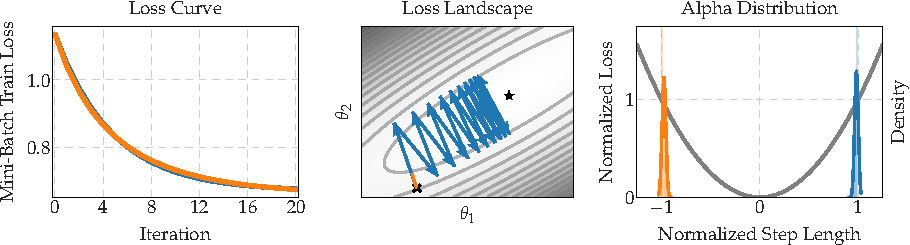
\includegraphics{../repos/cockpit-paper/fig/02_LINE/output/LINE_thesis-wide}
  \caption{\textbf{Illustrative example: learning curves do not tell the whole
      story}. Two different optimization runs
    (\textcolor{sns_orange}{\textbf{---}}/\textcolor{sns_blue}{\textbf{---}})
    can lead to virtually the same loss curve (\textit{left}). However, the
    actual optimization trajectories (\textit{middle}), exhibit vastly different
    behaviors. In practice, the trajectories are intractably large and cannot be
    visualized directly. Recommendable actions for both scenarios
    (\textcolor{sns_orange}{increase}/\textcolor{sns_blue}{decrease} the
    learning rate) cannot be inferred from the loss curve. The
    $\alpha$-distribution, one \cockpit instrument (\textit{right}), not only
    clearly distinguishes the two scenarios, but also allows for taking
    decisions how the learning rate should be adapted. See
    \Cref{cockpit::sec:alpha_exp} for further details.}\label{cockpit::fig:LINE}
\end{figure*}

\begin{figure*}[!t]
  \centering
  % trim={<left> <lower> <right> <upper>}, clip
  \Cshadowbox{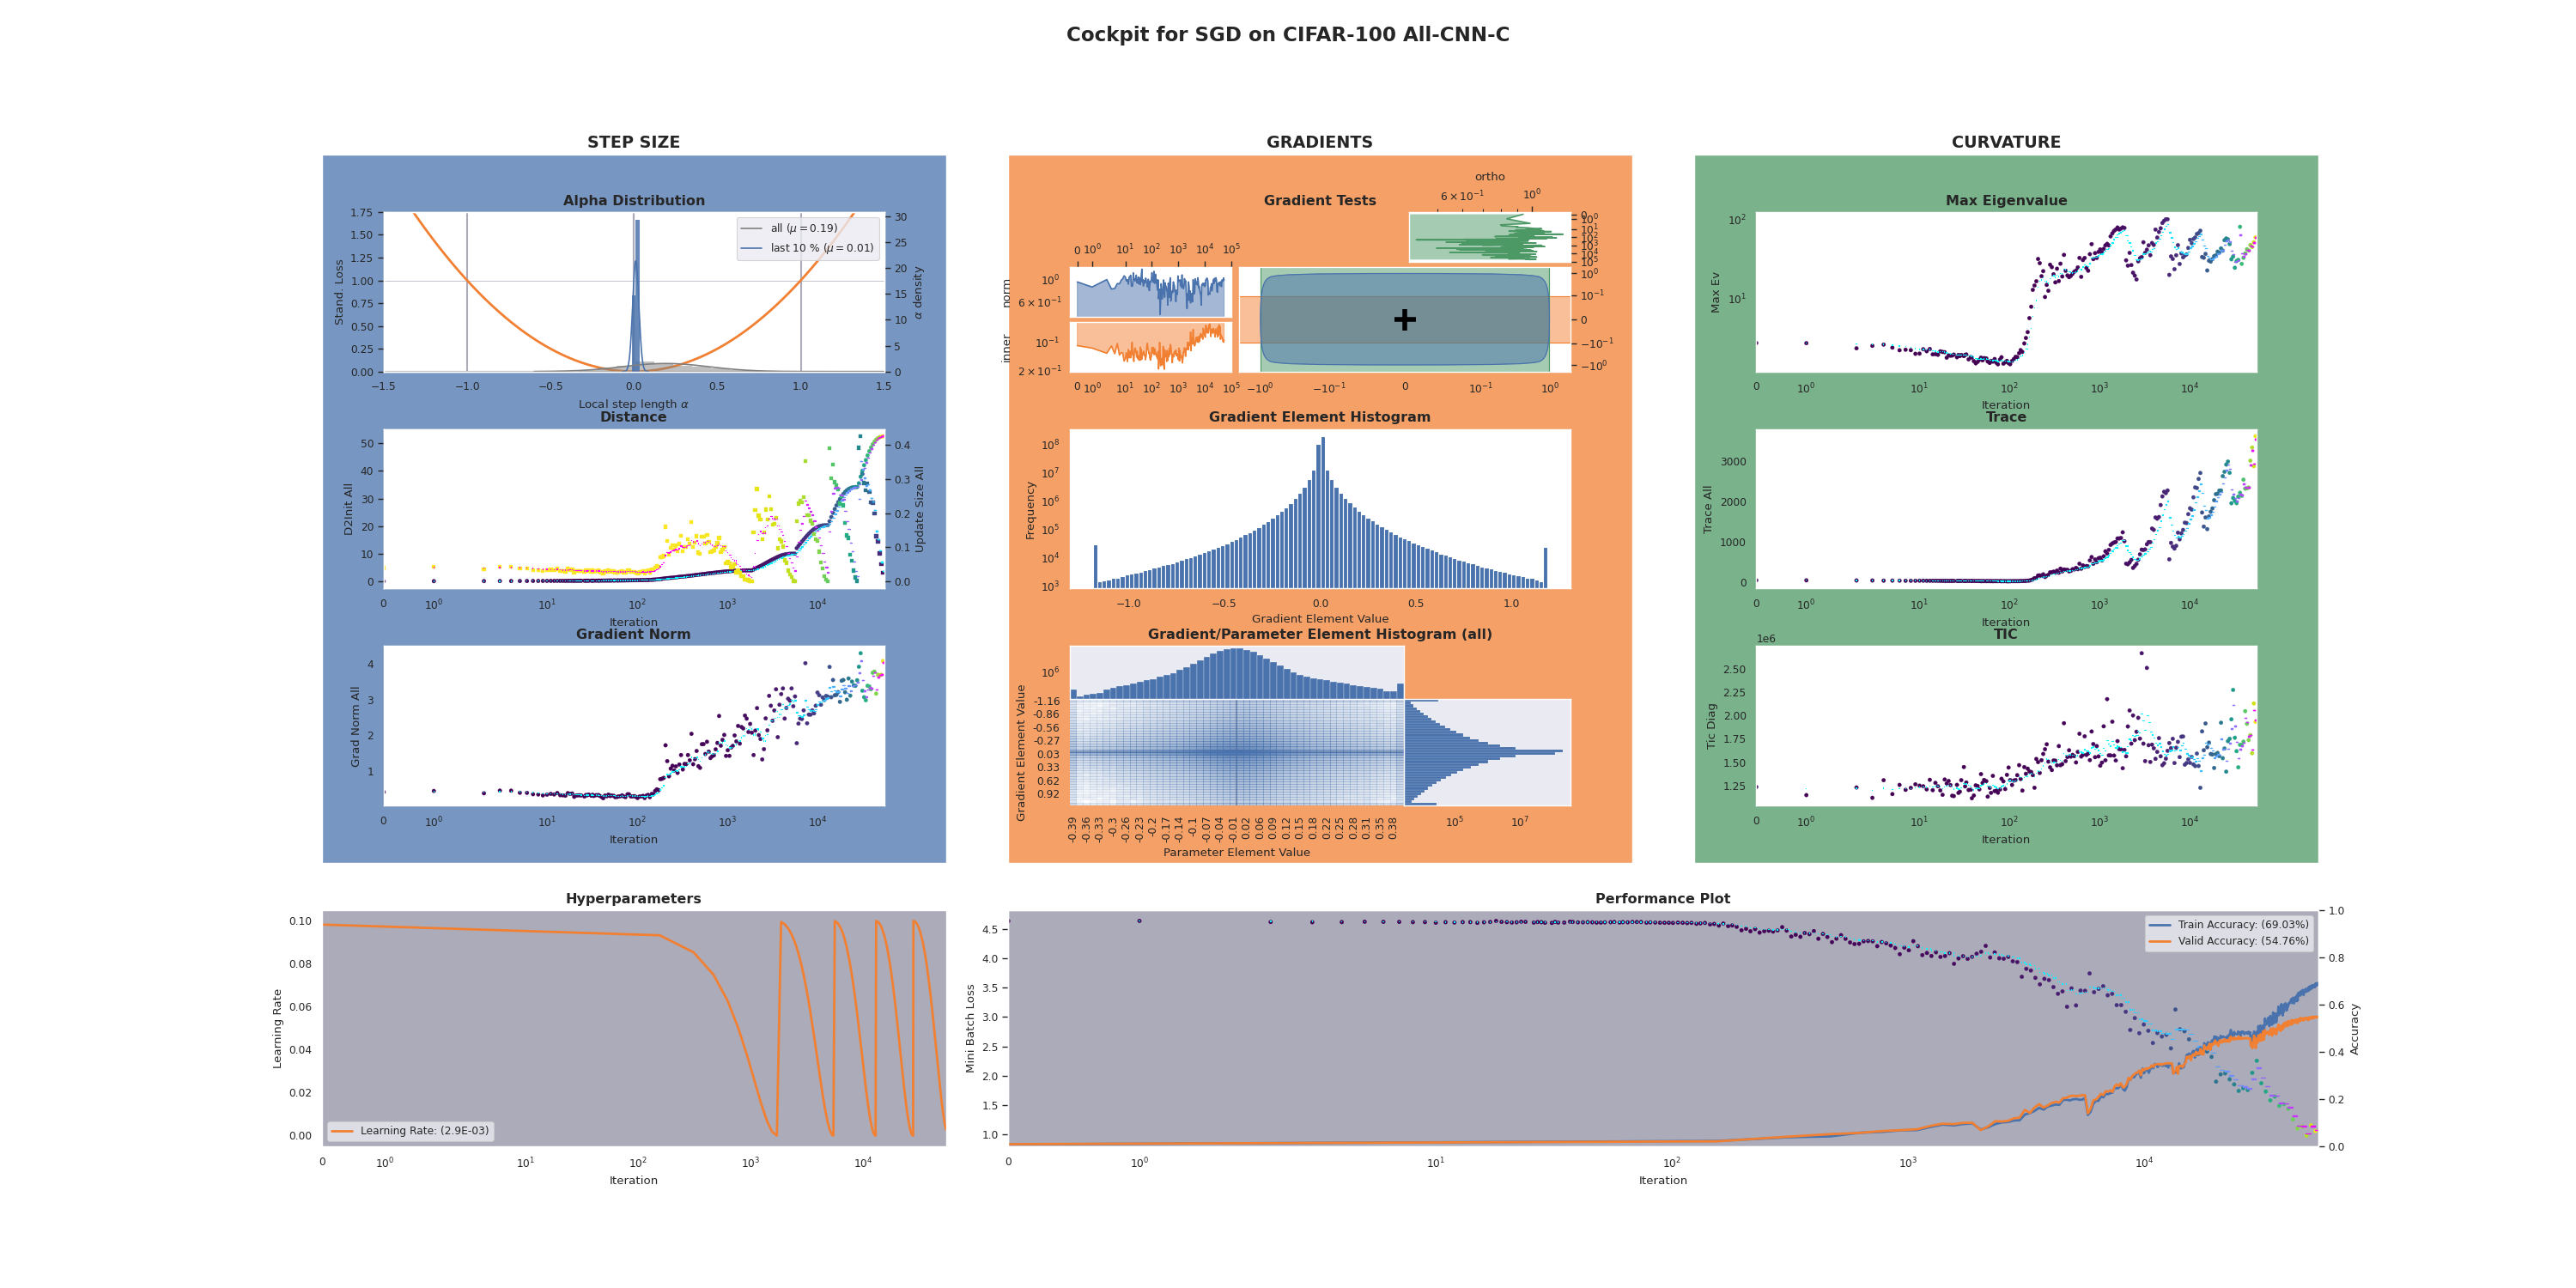
\includegraphics[width=0.97\linewidth, trim={7cm 2.5cm 5cm
      0.5cm}, clip]{../repos/cockpit-paper/tex/fig/10_showcase/cifar100_allcnnc_log.png}}
  \vspace{0.5ex}
  \caption{\textbf{Screenshot of \cockpittitle's full view} while training the
    \allcnnc \citep{springenberg2015striving} on \cifarhun with \sgd using a cyclical
    learning rate schedule. This figure and its labels are not meant to be
    legible, but rather give an impression of \cockpit's user experience. Gray
    panels (bottom row) show the information currently tracked by most
    practitioners. The individual instruments are discussed in
    \Cref{cockpit::sec:instruments}, and observations are described in
    \Cref{cockpit::sec:showcase}. An animated version can be found in the accompanying
    Github repository.}
  \label{cockpit::fig:showcase}
\end{figure*}

We aim to enrich the deep learning pipeline with a visual and statistical
debugging tool that uses newly proposed observables as well as several
established ones (\Cref{cockpit::sec:instruments}). We leverage and augment recent
extensions to AD (\ie \backpack \citep{dangel2020backpack} for
\pytorch \citep{paszke2019pytorch}) to efficiently access second-order statistical (\eg
gradient variances) and geometric (\eg Hessian) information. We show how these
quantities can aid the deep learning engineer in tasks, like learning rate
selection, as well as detecting common bugs with data processing or model
architectures (\Cref{cockpit::sec:experiments}).

Concretely, we introduce \cockpit, a flexible and efficient framework for
online-monitoring these observables during training in carefully designed plots
we call ``instruments'' (\Cref{cockpit::fig:showcase}). To practical, such
visualization must have a manageable computational overhead. We show that
\cockpit scales well to real-world deep learning problems (see
\Cref{cockpit::fig:showcase} and \Cref{cockpit::sec:showcase}). We also provide
three different configurations of varying computational complexity and
demonstrate that their instruments keep the computational cost \textit{well
  below} a factor of $2$ in run time (\Cref{cockpit::sec:benchmark}). It is
available as open-source code, extendable, and seamlessly integrates into
existing \pytorch training loops (\Cref{cockpit::app:code_example}).

%%% Local Variables:
%%% mode: latex
%%% TeX-master: "../thesis"
%%% End:


\section{\cockpittitle's Instruments}\label{cockpit::sec:instruments}
\subsubsection{Setting}

We consider supervised regression/classification with labeled data $(\vx, \vy)
\in \sX \times \sY$ generated by a distribution $\pdata(\vx, \vy)$. The training
set $\sD = \{ (\vx_n, \vy_n)\}_{n=1}^N$ consists of $N$ \iid samples from
$\pdata$ and the deep model $f_{\vtheta}: \sX \rightarrow \sF$ maps inputs
$\vx_n$ to predictions $f_{\vtheta}(\vx_n)$ by parameters $\vtheta \in \sTheta
:= \sR^D$. This prediction is evaluated by a loss function $\ell : \sF \times
\sY \rightarrow \R$ which compares to the label $\vy_n$. The goal is minimizing
an inaccessible expected risk $\gL_{\pdata}(\vtheta) = \int
\ell(f_{\vtheta}(\vx), \vy) \ \rd \pdata(\vx, \vy)$ by empirical approximation
through $\gL_{\sD}(\vtheta) = \nicefrac{1}{N} \sum_{n=1}^N
\ell(f_{\vtheta}(\vx_n), \vy_n) := \nicefrac{1}{N} \sum_{n=1}^N
\ell_n(\vtheta)$, which in practice is stochastically sub-sampled on
mini-batches $\sB \subset \sD$,
\begin{align}
  \label{cockpit::eq:mini-batch-loss}
  \gL_{\sB}(\vtheta) = \frac{1}{|\sB|} \sum_{(\vx_n,\vy_n) \in\sB} \ell_n(\vtheta)\,.
\end{align}
As is standard practice, we use first- and second-order information of the
mini-batch loss, described by its gradient $\vg_{\sB}(\vtheta)$ and Hessian
$\mH_{\sB}(\vtheta)$,
\begin{align}
  \vg_{\sB}(\vtheta)
  =
  \frac{1}{|\sB|} \sum_{(\vx_n, \vy_n) \in \sB}
  \grad{\vtheta}\ell_n(\vtheta)\, ,
  \quad
  \mH_{\sB}(\vtheta)
  =
  \frac{1}{|\sB|} \sum_{(\vx_n, \vy_n) \in \sB}
  \gradsquared{\vtheta} \ell_n(\vtheta)\,.
\end{align}

\subsubsection{Design Choices}

To minimize computational and design overhead, we restrict the metrics to
quantities that require no additional model evaluations. This means that, at
training step $t \to t + 1$ with mini-batches $\sB_t, \sB_{t+1}$ and parameters
$\vtheta_t, \vtheta_{t+1}$, we access information about the mini-batch losses
$\gL_{\sB_t}(\vtheta_t)$ and $\gL_{\sB_{t+1}}(\vtheta_{t+1})$, but no
cross-terms that require additional forward passes.

\subsubsection{Key Point}

$\gL_{\sB}(\vtheta), \vg_{\sB}(\vtheta)$, and $\mH_{\sB}(\vtheta)$ are just
expected values of a \textit{distribution} over the batch. Only recently, this
distribution has begun to attract attention \citep{faghri2020study} as its
computation has become more accessible \citep{bradbury2018jax,
  dangel2020backpack}. Contemporary optimizers leverage only the \emph{mean}
gradient and neglect higher moments. One core point of our work is making
extensive use of these distribution properties, trying to visualize them in
various ways. This distinguishes \cockpit from being ``just a collection of
plots'' that could be built in tools like \tensorboard. Leveraging these
distributional quantities, we create instruments and show how they can help
adapt hyperparameters (\Cref{cockpit::sec:adapting_hyperparameters}), analyze
the loss landscape (\Cref{cockpit::sec:curvature}), and track network dynamics
(\Cref{cockpit::sec:network_dynamics}). Instruments can sometimes be built from
already-computed information or are efficient variants of previously proposed
observables. To keep the presentation concise, we highlight the instruments
shown in \Cref{cockpit::fig:showcase} and listed in
\Cref{cockpit::tab:overview-quantities}. \Cref{cockpit::app:instruments} defines
them formally and contains more extensions, such as the mean \gsnr
\citep{liu2020understanding}, the early stopping \citep{mahsereci2017early} and
\cabs \citep{balles2017coupling} criterion, which can all be used in \cockpit.

{\def\arraystretch{1.2}
  \begin{table*}
    \caption{\textbf{Overview of \cockpittitle quantities}. They range from
      cheap byproducts, to nonlinear transformations of first-order information
      and Hessian-based measures. Some quantities have already been proposed,
      others are first to be considered in this work. They are categorized into
      configurations \textit{economy $\subseteq$ business $\subseteq$ full} based on their
      run time overhead (see \Cref{cockpit::sec:benchmark} for a detailed evaluation).}
    \label{cockpit::tab:overview-quantities}
    \begin{center}
      \footnotesize
      \begin{tabularx}{\linewidth}{lXcr}
        \toprule
        \textbf{Name}       & \textbf{Short Description}                                                                                           & \textbf{Config}   & \textbf{Pos.\,in Fig.\,\ref{cockpit::fig:showcase}}  \\
        \midrule
        \inlinecode{Alpha}      & Normalized step size on a noisy quadratic interpolation between $\vtheta_t$, $\vtheta_{t+1}$            & \textit{economy}  & top \textcolor{sns_blue}{left}        \\
        \inlinecode{Distance}   & Distance from initialization $\lVert \vtheta_{t} -  \vtheta_{0}  \rVert_2$                                           & \textit{economy}  & middle \textcolor{sns_blue}{left}     \\
        \inlinecode{UpdateSize} & Update size $\lVert \vtheta_{t + 1} - \vtheta_{t} \rVert_2$                                                          & \textit{economy}  & middle \textcolor{sns_blue}{left}     \\
        \inlinecode{GradNorm}   & Mini-batch gradient norm $\lVert \vg_{\sB}(\vtheta) \rVert_2$                                                        & \textit{economy}  & bottom \textcolor{sns_blue}{left}     \\
        \inlinecode{NormTest}   & Normalized fluctuations of residual norms ${\lVert  \vg_{\sB} - \vg_n \rVert_2}$, proposed in \citep{byrd2012sample}   & \textit{economy}  & top \textcolor{sns_orange}{center}    \\
        \inlinecode{InnerTest}  & Normalized fluctuations of $\vg_n$'s parallel to $\vg_{\sB}$, proposed in \citep{bollapragada2017adaptive} & \textit{economy}  & top \textcolor{sns_orange}{center}    \\
        \inlinecode{OrthoTest}  & Like  \inlinecode{InnerTest} but using the orthogonal components, proposed in \citep{bollapragada2017adaptive}                 & \textit{economy}  & top \textcolor{sns_orange}{center}    \\
        \inlinecode{GradHist1d} & Histogram of individual gradient elements, $\{[\vg_n]_j\}_{(\vx_{n},
                              \vy_{n}) \in \sB}^{j=1,\dots,D}$                           & \textit{economy}  & middle \textcolor{sns_orange}{center} \\
        \inlinecode{TICDiag}    & Relation of (diagonal) curvature and gradient noise, inspired by \citep{thomas2020interplay}                             & \textit{business} & bottom \textcolor{sns_green}{right}   \\
        \inlinecode{HessTrace}  & Exact or approximate Hessian trace, $\Tr(\mH_{\sB}(\vtheta))$, inspired by \citep{yao2020pyhessian}                           & \textit{business} & middle \textcolor{sns_green}{right}   \\
        \inlinecode{HessMaxEV}  & Maximum Hessian eigenvalue, $\lambda_{\text{max}}(\mH_{\sB}(\vtheta))$, inspired by \citep{yao2020pyhessian}                  & \textit{full}     & top \textcolor{sns_green}{right}      \\
        \inlinecode{GradHist2d} & Histogram of weights \& per-sample gradients, $\{
                              (\evtheta_j,[\vg_n]_j)\}_{(\vx_{n},
                              \vy_{n}) \in \sB}^{j=1,\dots,D}$  & \textit{full}     & bottom \textcolor{sns_orange}{center} \\
        \bottomrule
      \end{tabularx}
    \end{center}
  \end{table*}
}

%%% Local Variables:
%%% mode: latex
%%% TeX-master: "../../thesis"
%%% End:


\subsection{Adapting Hyperparameters}\label{cockpit::sec:adapting_hyperparameters}
One big challenge in deep learning is setting the hyperparameters correctly,
which is currently mostly done by trial \& error through parameter searches. We
aim to augment this process with instruments that inform the user about the
effect that the chosen parameters have on the current training process.

\subsubsection{\robustInlinecode{Alpha}: Are We Crossing the Valley?}

Using individual loss and gradient observations at the start and end point of
each iteration, we build a noise-informed uni-variate quadratic approximation
along the step direction (\ie the loss as a function of the step size), and
assess to which point on this parabola our optimizer moves. We standardize this
value $\alpha$ such that stepping to the valley-floor is assigned $\alpha=0$,
the starting point is at $\alpha=-1$ and updates to the point exactly opposite
of the starting point have $\alpha=1$ (see \Cref{cockpit::app:alpha} for a more
detailed visual and mathematical description of $\alpha$).
\Cref{cockpit::fig:LINE} illustrates the scenarios $\alpha=\pm1$ and how
monitoring the $\alpha$-distribution (right panel) can help distinguish between
two training runs with similar performance but distinct failure sources. By
default, this \cockpit instrument shows the $\alpha$-distribution for the last
10\,\% of training and the entire training process (top left plot in
\Cref{cockpit::fig:showcase}). In \Cref{cockpit::sec:alpha_exp} we show
empirically that, \emph{counter-intuitively}, it is generally \emph{not} a good
idea to choose the step size such that $\alpha$ is close to zero.

\subsubsection{Distances: Are We Making Progress?}

Another way to discern the trajectories in \Cref{cockpit::fig:LINE} is by
measuring the $L_2$ \textit{distance from initialization}
\citep{nagarajan2019generalization} and the \textit{update size}
\citep{agrawal2020investigating,frankle2020early} in parameter space. Both are
shown together in one \cockpit instrument (see also center-left plot in
\Cref{cockpit::fig:showcase}) and are far larger for the blue line in
\Cref{cockpit::fig:LINE}. These distance metrics are also able to disentangle
phases for the blue path. Using the same step size, it will continue to ``jump
back and forth'' between the loss valley's walls but at some point cease to make
progress. During this ``surfing of the walls'', the \textit{distance from
  initialization} increases, ultimately though, it will stagnate, with the
\textit{update size} remaining non-zero, indicating diffusion. While the initial
``surfing the wall''-phase benefits training (see
\Cref{cockpit::sec:alpha_exp}), achieving stationarity may require adaptation
once the optimizer reaches that diffusion.

\subsubsection{Gradient Norm: How Steep Is the Wall?}

The \textit{update size} will show that the orange trajectory is stuck. But why?
Such slow-down can result from both a bad learning rate and from loss landscape
plateaus. The \textit{gradient norm} (bottom left panel in
\Cref{cockpit::fig:showcase}) distinguishes these two causes.

\subsubsection{Gradient Tests: How Noisy Is the Batch?}

The batch size trades off gradient accuracy versus computational cost. Recently,
adaptive sampling strategies based on testing geometric constraints between mean
and individual gradients have been proposed
\citep{byrd2012sample,bollapragada2017adaptive}. The \textit{norm},
\textit{inner product}, and \textit{orthogonality tests} use a standardized
radius and two band widths (parallel and orthogonal to the gradient mean) that
indicate how strongly individual gradients scatter around the mean. The original
works use these values to adapt batch sizes. Instead, \cockpit combines all
three tests into a single gauge (top middle plot of
\Cref{cockpit::fig:showcase}) using the standardized noise radius and band
widths for visualization. These noise signals can be used to guide batch size
adaptation on- and offline, or to probe the influence of gradient alignment on
training speed \citep{sankararaman2020impact} and generalization
\citep{chatterjee2020coherent,chatterjee2020making,liu2020understanding}.

\subsection{Hessian Properties for Local Loss Geometry}\label{cockpit::sec:curvature}
An intuition for the local loss landscape helps in many ways. It can help
diagnose whether training is stuck, to adapt the step size, and explain
stability or regularization \citep{ginsburg2020regularization,jastrzebski2020break}. The key
challenge is the large number of weights: low-dimensional projections of
surfaces can behave unintuitively \citep{mulayoff2020unique}, but tracking the extreme
or average behaviors may help in debugging, especially if first-order metrics
fail.

\subsubsection{Hessian Eigenvalues: A Gorge or a Lake?}

In convex optimization, the maximum Hessian eigenvalue crucially determines the
appropriate step size \citep{schmidt2014convergence}. Many works have studied
the Hessian spectrum in machine learning
\citep[\eg][]{ghorbani2019investigation,ginsburg2020regularization,mulayoff2020unique,sagun2017eigenvalues,sagun2018empirical,yao2020pyhessian}.
In short: curvature matters. Established \citep{pearlmutter1994fast} and recent
autodiff frameworks \citep{dangel2020backpack} can compute Hessian properties
without requiring the full matrix. \cockpit leverages this to provide the
\textit{Hessian's largest eigenvalue} and \textit{trace} (right top and middle
plots in \Cref{cockpit::fig:showcase}). The former resembles the loss surface's
sharpest valley and can thus hint at training instabilities
\citep{jastrzebski2020break}. The \textit{trace} describes a notion of ``average
curvature'', since the eigenvalues $\lambda_i$ relate to it by $\sum_i \lambda_i
= \Tr(\mH_{\sB}(\vtheta))$, which might correlate with generalization
\citep{jastrzebski2021catastrophic}.

\subsubsection{TIC: How Do Curvature \& Gradient Noise Interact?}

There is an ongoing debate about curvature's link to generalization
\citep[\eg][]{dinh2017sharp,hochreiter1997flat,keskar2017large}. The
\emph{Takeuchi Information Criterion (TIC)}
\citep{takeuchi1976distribution,thomas2020interplay} estimates the
generalization gap by a ratio between Hessian and non-central second gradient
moment. It also provides intuition for changes in the objective function implied
by gradient noise. Inspired by \cite{thomas2020interplay}, \cockpit provides mini-batch TIC estimates (bottom
right plot of \Cref{cockpit::fig:showcase}).

\subsection{Visualizing Internal Network Dynamics}\label{cockpit::sec:network_dynamics}
Histograms are a natural visual compression of the high-dimensional $|\sB|
\times D$ individual gradient values. They give insights into the gradient
\emph{distribution} and hence offer a more detailed view of the learning signal.
Together with the parameter associated to each individual gradient, the entire
model status and dynamics can be visualized in a single plot and be monitored
during training. This provides a more fine-grained view of training compared to
tracking parameters and gradient norms \citep{frankle2020early}.

\subsubsection{Gradient \& Parameter Histograms: What Is Happening in Our Net?}

\cockpit offers a uni-variate \textit{histogram of the gradient elements}, \ie
the numbers
$\{[\vg_n( \vtheta )]_j\}_{(\vx_{n}, \vy_{n})\in \sB}^{j=1,\dots,D}$.
Additionally, a combined \textit{histogram of parameter-gradient pairs}
$\{([\vtheta]_j, [\vg_n( \vtheta )]_j\}_{(\vx_{n}, \vy_{n})\in \sB}^{j=1,\dots,D}$
provides a two-dimensional look into the network's gradient and parameter values
in a mini-batch. \Cref{cockpit::sec:misscaled_data_exp} shows an example
use-case of the gradient histogram; \Cref{cockpit::sec:vanishing_gradient_exp}
makes the case for the layer-wise variants of the instruments.

%%% Local Variables:
%%% mode: latex
%%% TeX-master: "../thesis"
%%% End:


\section{Experiments}\label{cockpit::sec:experiments}
The diverse information provided by \cockpit can help users and researchers in
many ways, some of which, just like for a traditional debugger, only become
apparent in practical use. In this section, we present a few motivating
examples, selecting specific instruments and scenarios in which they are
practically useful. Specifically, we show that \cockpit can help the user
discern between, and thus fix, common training bugs
(\Cref{cockpit::sec:misscaled_data_exp,cockpit::sec:vanishing_gradient_exp}) that are otherwise
hard to distinguish as they lead to the same failure: bad training. We
demonstrate that \cockpit can guide practitioners to choose efficient
hyperparameters \emph{within a single training run}
(\Cref{cockpit::sec:vanishing_gradient_exp,cockpit::sec:alpha_exp}). Finally, we highlight that
\cockpit's instruments can provide research insights about the optimization
process (\Cref{cockpit::sec:alpha_exp}). Our empirical findings are demonstrated on
problems from the \deepobs \citep{schneider2019deepobs} benchmark collection.

\subsection{Incorrectly Scaled Data}\label{cockpit::sec:misscaled_data_exp}
One prominent source of bugs is the data pipeline. To pick a relatively simple
example: for standard optimizers to work at their usual learning rates, network
inputs must be standardized (\ie~between zero and one, or have zero mean and
unit variance \citep[\eg][]{bengio2012neural}). If the user forgets to do this,
optimizer performance is likely to degrade. It can be difficult to identify the
source of this problem as it does not cause obvious failures, \texttt{NaN} or
\texttt{Inf} gradients, \etc. We now construct a semi-realistic example, to show
how using \cockpit can help diagnose this problem upon observing slow training
performance.

By default\sidenote{See the documentation, available at
  \href{https://www.cs.toronto.edu/~kriz/cifar.html}{\texttt{cs.toronto.edu/\textasciitilde
      kriz/cifar.html}}}, the popular image datasets \cifartenhun
\citep{krizhevsky2009learning} are provided as \numpy \citep{harris2020array}
arrays that consist of integers in the interval $[0,255]$. This \emph{raw} data,
instead of the widely used version with floats in $[0,1]$, changes the data
scale and thus the gradients by a factor of $255$. Therefore, the optimizer's
optimal learning rate is scaled as well. In other words, the default parameters
of popular optimization methods may not work well anymore, or good
hyperparameters may take extreme values. Even if the user directly inspects the
training images, this may not be apparent
(\Cref{cockpit::fig:data-pre-processing}). But the gradient histogram instrument
of \cockpit, which has a deliberate default plotting range around $[-1,1]$ to
highlight such problems, immediately and prominently shows that there is an
issue.

\begin{figure}
%	 pgfplots style "prerocessingexperimentdefault"
		\pgfkeys{/pgfplots/preprocessingexperimentdefault/.style={
				width=\linewidth,
				height=1.4\linewidth,
				every axis plot/.append style={line width = 1.2pt},
				tick pos = left,
				xmajorticks = true,
				ymajorticks = true,
				ylabel near ticks,
				xlabel near ticks,
				xtick align = inside,
				ytick align = inside,
				legend cell align = left,
				legend columns = 1,
				legend pos = south east,
				legend style = {
					fill opacity = 0.9,
					text opacity = 1,
					font = \small,
				},
				xticklabel style = {font = \small, inner xsep = -5ex},
				xlabel style = {font = \small},
				axis line style = {black},
				yticklabel style = {font = \small, inner ysep = -4ex},
				ylabel style = {font = \small},
				title style = {font = \small, inner ysep = -3ex},
				grid = major,
				grid style = {dashed}
			}
		}
	
	\centering
	\begin{subfigure}[t]{0.46\textwidth}
		\begin{minipage}{.49\textwidth}
			\Cshadowbox{
\includegraphics[width = .35\textwidth]{fig/06_preprocessing/fig_samples/cifar10raw_3c3d_sample_00.png}}
			\Cshadowbox{
\includegraphics[width = .35\textwidth]{fig/06_preprocessing/fig_samples/cifar10raw_3c3d_sample_01.png}}
	
			\Cshadowbox{
\includegraphics[width = .35\textwidth]{fig/06_preprocessing/fig_samples/cifar10raw_3c3d_sample_02.png}}
			\Cshadowbox{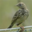
\includegraphics[width = .35\textwidth]{fig/06_preprocessing/fig_samples/cifar10raw_3c3d_sample_03.png}}
		\end{minipage}
		\begin{minipage}{.49\textwidth}
			\centering
			%			 customize "zmystyle" as you wish
			\pgfkeys{/pgfplots/zmystyle/.style={preprocessingexperimentdefault,
					ylabel={Gradient Element}
			}}
			\vspace{1.4\baselineskip}
			% This file was created by tikzplotlib v0.9.8.
\begin{tikzpicture}

\definecolor{color0}{rgb}{0.12156862745098,0.466666666666667,0.705882352941177}

\begin{axis}[
axis line style={white},
log basis x={10},
tick align=outside,
xmajorticks=false,
xmin=0.9, xmax=239494401.773689,
xmode=log,
xtick style={color=white!15!black},
ymajorticks=false,
ymin=-1.5, ymax=1.5,
zmystyle
]
\draw[draw=white,fill=color0,line width=0.04pt] (axis cs:0.9,-1.5) rectangle (axis cs:0.9,-1.42499995231628);
\draw[draw=white,fill=color0,line width=0.04pt] (axis cs:0.9,-1.42500007152557) rectangle (axis cs:0.9,-1.35000002384186);
\draw[draw=white,fill=color0,line width=0.04pt] (axis cs:0.9,-1.35000002384186) rectangle (axis cs:0.9,-1.27499997615814);
\draw[draw=white,fill=color0,line width=0.04pt] (axis cs:0.9,-1.27499997615814) rectangle (axis cs:0.9,-1.19999992847443);
\draw[draw=white,fill=color0,line width=0.04pt] (axis cs:0.9,-1.20000004768372) rectangle (axis cs:0.9,-1.125);
\draw[draw=white,fill=color0,line width=0.04pt] (axis cs:0.9,-1.125) rectangle (axis cs:0.9,-1.04999995231628);
\draw[draw=white,fill=color0,line width=0.04pt] (axis cs:0.9,-1.04999995231628) rectangle (axis cs:0.9,-0.974999904632568);
\draw[draw=white,fill=color0,line width=0.04pt] (axis cs:0.9,-0.975000023841858) rectangle (axis cs:0.9,-0.899999976158142);
\draw[draw=white,fill=color0,line width=0.04pt] (axis cs:0.9,-0.899999976158142) rectangle (axis cs:0.9,-0.824999928474426);
\draw[draw=white,fill=color0,line width=0.04pt] (axis cs:0.9,-0.825000047683716) rectangle (axis cs:0.9,-0.75);
\draw[draw=white,fill=color0,line width=0.04pt] (axis cs:0.9,-0.75) rectangle (axis cs:0.9,-0.674999952316284);
\draw[draw=white,fill=color0,line width=0.04pt] (axis cs:0.9,-0.674999952316284) rectangle (axis cs:0.9,-0.599999904632568);
\draw[draw=white,fill=color0,line width=0.04pt] (axis cs:0.9,-0.600000023841858) rectangle (axis cs:0.9,-0.524999976158142);
\draw[draw=white,fill=color0,line width=0.04pt] (axis cs:0.9,-0.524999976158142) rectangle (axis cs:0.9,-0.449999928474426);
\draw[draw=white,fill=color0,line width=0.04pt] (axis cs:0.9,-0.449999988079071) rectangle (axis cs:0.9,-0.374999940395355);
\draw[draw=white,fill=color0,line width=0.04pt] (axis cs:0.9,-0.374999970197678) rectangle (axis cs:0.9,-0.299999922513962);
\draw[draw=white,fill=color0,line width=0.04pt] (axis cs:0.9,-0.299999982118607) rectangle (axis cs:15.9,-0.224999934434891);
\draw[draw=white,fill=color0,line width=0.04pt] (axis cs:0.9,-0.224999964237213) rectangle (axis cs:755.9,-0.149999916553497);
\draw[draw=white,fill=color0,line width=0.04pt] (axis cs:0.9,-0.149999968707561) rectangle (axis cs:12866.9,-0.0749999210238457);
\draw[draw=white,fill=color0,line width=0.04pt] (axis cs:0.9,-0.075000025331974) rectangle (axis cs:95082889.9,2.23517417907715e-08);
\draw[draw=white,fill=color0,line width=0.04pt] (axis cs:0.9,-8.19563865661621e-08) rectangle (axis cs:19475047.9,0.0749999657273293);
\draw[draw=white,fill=color0,line width=0.04pt] (axis cs:0.9,0.0749999210238457) rectangle (axis cs:14378.9,0.149999968707561);
\draw[draw=white,fill=color0,line width=0.04pt] (axis cs:0.9,0.149999916553497) rectangle (axis cs:794.9,0.224999964237213);
\draw[draw=white,fill=color0,line width=0.04pt] (axis cs:0.9,0.224999934434891) rectangle (axis cs:8.9,0.299999982118607);
\draw[draw=white,fill=color0,line width=0.04pt] (axis cs:0.9,0.299999922513962) rectangle (axis cs:0.9,0.374999970197678);
\draw[draw=white,fill=color0,line width=0.04pt] (axis cs:0.9,0.374999940395355) rectangle (axis cs:0.9,0.449999988079071);
\draw[draw=white,fill=color0,line width=0.04pt] (axis cs:0.9,0.449999928474426) rectangle (axis cs:0.9,0.524999976158142);
\draw[draw=white,fill=color0,line width=0.04pt] (axis cs:0.9,0.524999976158142) rectangle (axis cs:0.9,0.600000023841858);
\draw[draw=white,fill=color0,line width=0.04pt] (axis cs:0.9,0.599999904632568) rectangle (axis cs:0.9,0.674999952316284);
\draw[draw=white,fill=color0,line width=0.04pt] (axis cs:0.9,0.674999952316284) rectangle (axis cs:0.9,0.75);
\draw[draw=white,fill=color0,line width=0.04pt] (axis cs:0.9,0.75) rectangle (axis cs:0.9,0.825000047683716);
\draw[draw=white,fill=color0,line width=0.04pt] (axis cs:0.9,0.824999928474426) rectangle (axis cs:30.9,0.899999976158142);
\draw[draw=white,fill=color0,line width=0.04pt] (axis cs:0.9,0.899999976158142) rectangle (axis cs:98.9,0.975000023841858);
\draw[draw=white,fill=color0,line width=0.04pt] (axis cs:0.9,0.974999904632568) rectangle (axis cs:0.9,1.04999995231628);
\draw[draw=white,fill=color0,line width=0.04pt] (axis cs:0.9,1.04999995231628) rectangle (axis cs:0.9,1.125);
\draw[draw=white,fill=color0,line width=0.04pt] (axis cs:0.9,1.125) rectangle (axis cs:0.9,1.20000004768372);
\draw[draw=white,fill=color0,line width=0.04pt] (axis cs:0.9,1.19999992847443) rectangle (axis cs:0.9,1.27499997615814);
\draw[draw=white,fill=color0,line width=0.04pt] (axis cs:0.9,1.27499997615814) rectangle (axis cs:0.9,1.35000002384186);
\draw[draw=white,fill=color0,line width=0.04pt] (axis cs:0.9,1.35000002384186) rectangle (axis cs:0.9,1.42500007152557);
\draw[draw=white,fill=color0,line width=0.04pt] (axis cs:0.9,1.42499995231628) rectangle (axis cs:0.9,1.5);
\end{axis}

\end{tikzpicture}

		\end{minipage}
		\caption{Normalized Data}
		\label{fig:data-pre-processing_norm}
	\end{subfigure}
	\hfill
	\begin{subfigure}[t]{0.46\textwidth}
		\begin{minipage}{.49\textwidth}
			\Cshadowbox{
\includegraphics[width = .35\textwidth]{fig/06_preprocessing/fig_samples/cifar10scale255_3c3d_sample_00.png}}
			\Cshadowbox{
\includegraphics[width = .35\textwidth]{fig/06_preprocessing/fig_samples/cifar10scale255_3c3d_sample_01.png}}
			
			\Cshadowbox{
\includegraphics[width = .35\textwidth]{fig/06_preprocessing/fig_samples/cifar10scale255_3c3d_sample_02.png}}
			\Cshadowbox{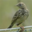
\includegraphics[width = .35\textwidth]{fig/06_preprocessing/fig_samples/cifar10scale255_3c3d_sample_03.png}}
		\end{minipage}
		\begin{minipage}{.49\textwidth}
			\centering
%			 customize "zmystyle" as you wish
			\pgfkeys{/pgfplots/zmystyle/.style={preprocessingexperimentdefault,
					ylabel={Gradient Element}
			}}
			\vspace{1.4\baselineskip}
			% This file was created by tikzplotlib v0.9.8.
\begin{tikzpicture}

\definecolor{color0}{rgb}{1,0.498039215686275,0.0549019607843137}

\begin{axis}[
axis line style={white},
log basis x={10},
tick align=outside,
xmajorticks=false,
xmin=0.9, xmax=199565229.367149,
xmode=log,
xtick style={color=white!15!black},
ymajorticks=false,
ymin=-1.5, ymax=1.5,
zmystyle
]
\draw[draw=white,fill=color0,line width=0.04pt] (axis cs:0.9,-1.5) rectangle (axis cs:6792656.9,-1.42499995231628);
\draw[draw=white,fill=color0,line width=0.04pt] (axis cs:0.9,-1.42500007152557) rectangle (axis cs:304537.9,-1.35000002384186);
\draw[draw=white,fill=color0,line width=0.04pt] (axis cs:0.9,-1.35000002384186) rectangle (axis cs:322920.9,-1.27499997615814);
\draw[draw=white,fill=color0,line width=0.04pt] (axis cs:0.9,-1.27499997615814) rectangle (axis cs:342177.9,-1.19999992847443);
\draw[draw=white,fill=color0,line width=0.04pt] (axis cs:0.9,-1.20000004768372) rectangle (axis cs:365697.9,-1.125);
\draw[draw=white,fill=color0,line width=0.04pt] (axis cs:0.9,-1.125) rectangle (axis cs:389812.9,-1.04999995231628);
\draw[draw=white,fill=color0,line width=0.04pt] (axis cs:0.9,-1.04999995231628) rectangle (axis cs:417003.9,-0.974999904632568);
\draw[draw=white,fill=color0,line width=0.04pt] (axis cs:0.9,-0.975000023841858) rectangle (axis cs:446173.9,-0.899999976158142);
\draw[draw=white,fill=color0,line width=0.04pt] (axis cs:0.9,-0.899999976158142) rectangle (axis cs:476860.9,-0.824999928474426);
\draw[draw=white,fill=color0,line width=0.04pt] (axis cs:0.9,-0.825000047683716) rectangle (axis cs:514596.9,-0.75);
\draw[draw=white,fill=color0,line width=0.04pt] (axis cs:0.9,-0.75) rectangle (axis cs:555044.9,-0.674999952316284);
\draw[draw=white,fill=color0,line width=0.04pt] (axis cs:0.9,-0.674999952316284) rectangle (axis cs:601849.9,-0.599999904632568);
\draw[draw=white,fill=color0,line width=0.04pt] (axis cs:0.9,-0.600000023841858) rectangle (axis cs:653348.9,-0.524999976158142);
\draw[draw=white,fill=color0,line width=0.04pt] (axis cs:0.9,-0.524999976158142) rectangle (axis cs:715926.9,-0.449999928474426);
\draw[draw=white,fill=color0,line width=0.04pt] (axis cs:0.9,-0.449999988079071) rectangle (axis cs:790634.9,-0.374999940395355);
\draw[draw=white,fill=color0,line width=0.04pt] (axis cs:0.9,-0.374999970197678) rectangle (axis cs:880821.9,-0.299999922513962);
\draw[draw=white,fill=color0,line width=0.04pt] (axis cs:0.9,-0.299999982118607) rectangle (axis cs:996047.9,-0.224999934434891);
\draw[draw=white,fill=color0,line width=0.04pt] (axis cs:0.9,-0.224999964237213) rectangle (axis cs:1158251.9,-0.149999916553497);
\draw[draw=white,fill=color0,line width=0.04pt] (axis cs:0.9,-0.149999968707561) rectangle (axis cs:1410941.9,-0.0749999210238457);
\draw[draw=white,fill=color0,line width=0.04pt] (axis cs:0.9,-0.075000025331974) rectangle (axis cs:79921533.9,2.23517417907715e-08);
\draw[draw=white,fill=color0,line width=0.04pt] (axis cs:0.9,-8.19563865661621e-08) rectangle (axis cs:1965478.9,0.0749999657273293);
\draw[draw=white,fill=color0,line width=0.04pt] (axis cs:0.9,0.0749999210238457) rectangle (axis cs:1289789.9,0.149999968707561);
\draw[draw=white,fill=color0,line width=0.04pt] (axis cs:0.9,0.149999916553497) rectangle (axis cs:1043170.9,0.224999964237213);
\draw[draw=white,fill=color0,line width=0.04pt] (axis cs:0.9,0.224999934434891) rectangle (axis cs:885990.9,0.299999982118607);
\draw[draw=white,fill=color0,line width=0.04pt] (axis cs:0.9,0.299999922513962) rectangle (axis cs:771669.9,0.374999970197678);
\draw[draw=white,fill=color0,line width=0.04pt] (axis cs:0.9,0.374999940395355) rectangle (axis cs:683281.9,0.449999988079071);
\draw[draw=white,fill=color0,line width=0.04pt] (axis cs:0.9,0.449999928474426) rectangle (axis cs:610831.9,0.524999976158142);
\draw[draw=white,fill=color0,line width=0.04pt] (axis cs:0.9,0.524999976158142) rectangle (axis cs:553292.9,0.600000023841858);
\draw[draw=white,fill=color0,line width=0.04pt] (axis cs:0.9,0.599999904632568) rectangle (axis cs:502804.9,0.674999952316284);
\draw[draw=white,fill=color0,line width=0.04pt] (axis cs:0.9,0.674999952316284) rectangle (axis cs:461496.9,0.75);
\draw[draw=white,fill=color0,line width=0.04pt] (axis cs:0.9,0.75) rectangle (axis cs:423747.9,0.825000047683716);
\draw[draw=white,fill=color0,line width=0.04pt] (axis cs:0.9,0.824999928474426) rectangle (axis cs:392145.9,0.899999976158142);
\draw[draw=white,fill=color0,line width=0.04pt] (axis cs:0.9,0.899999976158142) rectangle (axis cs:363396.9,0.975000023841858);
\draw[draw=white,fill=color0,line width=0.04pt] (axis cs:0.9,0.974999904632568) rectangle (axis cs:335621.9,1.04999995231628);
\draw[draw=white,fill=color0,line width=0.04pt] (axis cs:0.9,1.04999995231628) rectangle (axis cs:312992.9,1.125);
\draw[draw=white,fill=color0,line width=0.04pt] (axis cs:0.9,1.125) rectangle (axis cs:291497.9,1.20000004768372);
\draw[draw=white,fill=color0,line width=0.04pt] (axis cs:0.9,1.19999992847443) rectangle (axis cs:273292.9,1.27499997615814);
\draw[draw=white,fill=color0,line width=0.04pt] (axis cs:0.9,1.27499997615814) rectangle (axis cs:255338.9,1.35000002384186);
\draw[draw=white,fill=color0,line width=0.04pt] (axis cs:0.9,1.35000002384186) rectangle (axis cs:240647.9,1.42500007152557);
\draw[draw=white,fill=color0,line width=0.04pt] (axis cs:0.9,1.42499995231628) rectangle (axis cs:4873580.9,1.5);
\end{axis}

\end{tikzpicture}

		\end{minipage}
		\caption{Raw Data}
		\label{fig:data-pre-processing_raw}
	\end{subfigure}
	\caption{\textbf{Same inputs, different gradients; Catching data 
	    bugs with \cockpittitle.} (a) \emph{normalized} ($[0, 1]$) and (b)
    	\emph{raw} $([0, 255])$ images look identical in auto-scaled
	    front-ends like \matplotlib's \texttt{imshow}. The gradient distribution on
	    the \threecthreed model, however, is crucially affected by this
	    scaling.}
	\label{fig:data-pre-processing}
\end{figure}

%%% Local Variables:
%%% mode: latex
%%% TeX-master: "../cockpit_paper"
%%% End:


Of course, this particular data is only a placeholder for real practical data
sets. While this problem may not frequently arise in the highly pre-processed,
packaged \cifarten, it is not a rare problem for practitioners who work with
their personal datasets. This is particularly likely in domains outside
standard computer vision, \eg when working with mixed-type data without obvious
natural scales.

\subsection{Vanishing Gradients}\label{cockpit::sec:vanishing_gradient_exp}

The model itself can be a source of training bugs. As before, such problems
mostly arise with novel datasets, where well-working architectures are unknown.
The following example shows how even small (in terms of code) model
modifications may severely harm the training.

\Cref{cockpit::fig:layerwise-experiment_net} shows the distribution of gradient values of
two different network architectures in blue and orange. Although the blue model
trains considerably better than the orange one, their gradient distributions
look quite similar. The difference becomes evident when inspecting the histogram
\emph{layer-wise}. We can see that multiple layers have a degenerated gradient
distribution with many elements being practically zero (see
\Cref{cockpit::fig:layerwise-experiment_layers}, bottom row). Since the fully connected
layers close to the output have far more parameters (a typical pattern of
convolutional networks), they dominate the network-wide histogram. This obscures
that a major part of the model is effectively unable to train.

\begin{figure}
%	 pgfplots style "layerwiseexperimentdefault"
	  \pgfkeys{/pgfplots/layerwiseexperimentdefault/.style={
	      width=\linewidth,
	      height=0.13\textheight,
	      every axis plot/.append style={line width = 1.2pt},
	      tick pos = left,
	      xmajorticks = true,
	      ymajorticks = true,
	      ylabel near ticks,
	      xlabel near ticks,
	      xtick align = inside,
	      ytick align = inside,
	      ytick={-1,0,1},
	      legend cell align = left,
	      legend columns = 1,
	      legend pos = south east,
	      legend style = {
	        fill opacity = 0.9,
	        text opacity = 1,
	        font = \small,
	      },
	      xticklabel style = {font = \small, inner xsep = -5ex},
	      xlabel style = {font = \small},
	      axis line style = {black},
	      yticklabel style = {font = \small, inner ysep = -4ex},
	      ylabel style = {font = \small},
	      title style = {font = \small, inner ysep = -3ex},
	      grid = major,
	      grid style = {dashed}
	    }
	  }
	
	\centering
	\begin{subfigure}[t]{0.4\textwidth}
%		 customize "zmystyle" as you wish
		\pgfkeys{/pgfplots/zmystyle/.style={layerwiseexperimentdefault,
		   title = {Network}, ylabel=Gradient\\Element, ylabel style={align=left}, xticklabels = {}
		 }}
		% This file was created by tikzplotlib v0.9.8.
\begin{tikzpicture}

\definecolor{color0}{rgb}{0.12156862745098,0.466666666666667,0.705882352941177}

\begin{axis}[
axis line style={white},
log basis x={10},
tick align=outside,
xmajorticks=false,
xmin=0.9, xmax=233063278.37446,
xmode=log,
xtick style={color=white!15!black},
ymajorticks=false,
ymin=-1.1000000834465, ymax=1.1000000834465,
zmystyle
]
\draw[draw=white,fill=color0,line width=0.02pt] (axis cs:0.9,-1.1000000834465) rectangle (axis cs:0.9,-0.990000069141388);
\draw[draw=white,fill=color0,line width=0.02pt] (axis cs:0.9,-0.990000009536743) rectangle (axis cs:0.9,-0.879999995231628);
\draw[draw=white,fill=color0,line width=0.02pt] (axis cs:0.9,-0.880000054836273) rectangle (axis cs:0.9,-0.770000040531158);
\draw[draw=white,fill=color0,line width=0.02pt] (axis cs:0.9,-0.770000040531158) rectangle (axis cs:0.9,-0.660000026226044);
\draw[draw=white,fill=color0,line width=0.02pt] (axis cs:0.9,-0.660000026226044) rectangle (axis cs:0.9,-0.550000011920929);
\draw[draw=white,fill=color0,line width=0.02pt] (axis cs:0.9,-0.550000011920929) rectangle (axis cs:0.9,-0.439999997615814);
\draw[draw=white,fill=color0,line width=0.02pt] (axis cs:0.9,-0.440000057220459) rectangle (axis cs:23.9,-0.330000042915344);
\draw[draw=white,fill=color0,line width=0.02pt] (axis cs:0.9,-0.330000042915344) rectangle (axis cs:868.9,-0.220000028610229);
\draw[draw=white,fill=color0,line width=0.02pt] (axis cs:0.9,-0.220000028610229) rectangle (axis cs:38909.9,-0.110000014305115);
\draw[draw=white,fill=color0,line width=0.02pt] (axis cs:0.9,-0.110000006854534) rectangle (axis cs:92649650.9,7.45058059692383e-09);
\draw[draw=white,fill=color0,line width=0.02pt] (axis cs:0.9,2.23517417907715e-08) rectangle (axis cs:21858861.9,0.110000036656857);
\draw[draw=white,fill=color0,line width=0.02pt] (axis cs:0.9,0.110000014305115) rectangle (axis cs:35123.9,0.220000028610229);
\draw[draw=white,fill=color0,line width=0.02pt] (axis cs:0.9,0.220000028610229) rectangle (axis cs:2220.9,0.330000042915344);
\draw[draw=white,fill=color0,line width=0.02pt] (axis cs:0.9,0.330000042915344) rectangle (axis cs:686.9,0.440000057220459);
\draw[draw=white,fill=color0,line width=0.02pt] (axis cs:0.9,0.439999997615814) rectangle (axis cs:276.9,0.550000011920929);
\draw[draw=white,fill=color0,line width=0.02pt] (axis cs:0.9,0.550000011920929) rectangle (axis cs:95.9,0.660000026226044);
\draw[draw=white,fill=color0,line width=0.02pt] (axis cs:0.9,0.660000026226044) rectangle (axis cs:27.9,0.770000040531158);
\draw[draw=white,fill=color0,line width=0.02pt] (axis cs:0.9,0.770000040531158) rectangle (axis cs:25.9,0.880000054836273);
\draw[draw=white,fill=color0,line width=0.02pt] (axis cs:0.9,0.879999995231628) rectangle (axis cs:117.9,0.990000009536743);
\draw[draw=white,fill=color0,line width=0.02pt] (axis cs:0.9,0.990000069141388) rectangle (axis cs:0.9,1.1000000834465);
\end{axis}

\end{tikzpicture}

		
		\vspace{-0.1cm}
%		customize "zmystyle" as you wish
		\pgfkeys{/pgfplots/zmystyle/.style={layerwiseexperimentdefault,
		   ylabel=Gradient\\Element, ylabel style={align=left}
		 }}
		% This file was created by tikzplotlib v0.9.8.
\begin{tikzpicture}

\definecolor{color0}{rgb}{1,0.498039215686275,0.0549019607843137}

\begin{axis}[
axis line style={white},
log basis x={10},
tick align=outside,
xmajorticks=false,
xmin=0.9, xmax=141796339.435146,
xmode=log,
xtick style={color=white!15!black},
ymajorticks=false,
ymin=-1.1000000834465, ymax=1.1000000834465,
zmystyle
]
\draw[draw=white,fill=color0,line width=0.02pt] (axis cs:0.9,-1.1000000834465) rectangle (axis cs:0.9,-0.990000069141388);
\draw[draw=white,fill=color0,line width=0.02pt] (axis cs:0.9,-0.990000009536743) rectangle (axis cs:0.9,-0.879999995231628);
\draw[draw=white,fill=color0,line width=0.02pt] (axis cs:0.9,-0.880000054836273) rectangle (axis cs:0.9,-0.770000040531158);
\draw[draw=white,fill=color0,line width=0.02pt] (axis cs:0.9,-0.770000040531158) rectangle (axis cs:0.9,-0.660000026226044);
\draw[draw=white,fill=color0,line width=0.02pt] (axis cs:0.9,-0.660000026226044) rectangle (axis cs:0.9,-0.550000011920929);
\draw[draw=white,fill=color0,line width=0.02pt] (axis cs:0.9,-0.550000011920929) rectangle (axis cs:0.9,-0.439999997615814);
\draw[draw=white,fill=color0,line width=0.02pt] (axis cs:0.9,-0.440000057220459) rectangle (axis cs:116.9,-0.330000042915344);
\draw[draw=white,fill=color0,line width=0.02pt] (axis cs:0.9,-0.330000042915344) rectangle (axis cs:7658.9,-0.220000028610229);
\draw[draw=white,fill=color0,line width=0.02pt] (axis cs:0.9,-0.220000028610229) rectangle (axis cs:41443.9,-0.110000014305115);
\draw[draw=white,fill=color0,line width=0.02pt] (axis cs:0.9,-0.110000006854534) rectangle (axis cs:57718038.9,7.45058059692383e-09);
\draw[draw=white,fill=color0,line width=0.02pt] (axis cs:0.9,2.23517417907715e-08) rectangle (axis cs:56786753.9,0.110000036656857);
\draw[draw=white,fill=color0,line width=0.02pt] (axis cs:0.9,0.110000014305115) rectangle (axis cs:1065.9,0.220000028610229);
\draw[draw=white,fill=color0,line width=0.02pt] (axis cs:0.9,0.220000028610229) rectangle (axis cs:5071.9,0.330000042915344);
\draw[draw=white,fill=color0,line width=0.02pt] (axis cs:0.9,0.330000042915344) rectangle (axis cs:8560.9,0.440000057220459);
\draw[draw=white,fill=color0,line width=0.02pt] (axis cs:0.9,0.439999997615814) rectangle (axis cs:10133.9,0.550000011920929);
\draw[draw=white,fill=color0,line width=0.02pt] (axis cs:0.9,0.550000011920929) rectangle (axis cs:5885.9,0.660000026226044);
\draw[draw=white,fill=color0,line width=0.02pt] (axis cs:0.9,0.660000026226044) rectangle (axis cs:1847.9,0.770000040531158);
\draw[draw=white,fill=color0,line width=0.02pt] (axis cs:0.9,0.770000040531158) rectangle (axis cs:203.9,0.880000054836273);
\draw[draw=white,fill=color0,line width=0.02pt] (axis cs:0.9,0.879999995231628) rectangle (axis cs:108.9,0.990000009536743);
\draw[draw=white,fill=color0,line width=0.02pt] (axis cs:0.9,0.990000069141388) rectangle (axis cs:0.9,1.1000000834465);
\end{axis}

\end{tikzpicture}

		\caption{Network Histogram}
		\label{fig:layerwise-experiment_net}
	\end{subfigure}
	\hfill
	\begin{subfigure}[t]{0.57\textwidth}
		    \pgfkeys{/pgfplots/layerwiseexperimentdefaultparameters/.style={
		        layerwiseexperimentdefault,
		        ylabel={},
		        ylabel style = {inner ysep = -4ex},
		        yticklabels={},
		        width=0.45\textwidth,
		      }
		    }
		    \hfill%
		    \pgfkeys{/pgfplots/zmystyle/.style={layerwiseexperimentdefaultparameters,
		        title={Parameter 0}, xticklabels = {},}}%
		    % This file was created by tikzplotlib v0.9.8.
\begin{tikzpicture}

\definecolor{color0}{rgb}{0.12156862745098,0.466666666666667,0.705882352941177}

\begin{axis}[
axis line style={white},
log basis x={10},
tick align=outside,
xmajorticks=false,
xmin=0.9, xmax=570529.892272652,
xmode=log,
xtick style={color=white!15!black},
ymajorticks=false,
ymin=-1.1000000834465, ymax=1.1000000834465,
zmystyle
]
\draw[draw=white,fill=color0,line width=0.02pt] (axis cs:0.9,-1.1000000834465) rectangle (axis cs:0.9,-0.990000069141388);
\draw[draw=white,fill=color0,line width=0.02pt] (axis cs:0.9,-0.990000009536743) rectangle (axis cs:0.9,-0.879999995231628);
\draw[draw=white,fill=color0,line width=0.02pt] (axis cs:0.9,-0.880000054836273) rectangle (axis cs:0.9,-0.770000040531158);
\draw[draw=white,fill=color0,line width=0.02pt] (axis cs:0.9,-0.770000040531158) rectangle (axis cs:0.9,-0.660000026226044);
\draw[draw=white,fill=color0,line width=0.02pt] (axis cs:0.9,-0.660000026226044) rectangle (axis cs:0.9,-0.550000011920929);
\draw[draw=white,fill=color0,line width=0.02pt] (axis cs:0.9,-0.550000011920929) rectangle (axis cs:0.9,-0.439999997615814);
\draw[draw=white,fill=color0,line width=0.02pt] (axis cs:0.9,-0.440000057220459) rectangle (axis cs:23.9,-0.330000042915344);
\draw[draw=white,fill=color0,line width=0.02pt] (axis cs:0.9,-0.330000042915344) rectangle (axis cs:528.9,-0.220000028610229);
\draw[draw=white,fill=color0,line width=0.02pt] (axis cs:0.9,-0.220000028610229) rectangle (axis cs:11638.9,-0.110000014305115);
\draw[draw=white,fill=color0,line width=0.02pt] (axis cs:0.9,-0.110000006854534) rectangle (axis cs:301988.9,7.45058059692383e-09);
\draw[draw=white,fill=color0,line width=0.02pt] (axis cs:0.9,2.23517417907715e-08) rectangle (axis cs:288675.9,0.110000036656857);
\draw[draw=white,fill=color0,line width=0.02pt] (axis cs:0.9,0.110000014305115) rectangle (axis cs:11178.9,0.220000028610229);
\draw[draw=white,fill=color0,line width=0.02pt] (axis cs:0.9,0.220000028610229) rectangle (axis cs:370.9,0.330000042915344);
\draw[draw=white,fill=color0,line width=0.02pt] (axis cs:0.9,0.330000042915344) rectangle (axis cs:0.9,0.440000057220459);
\draw[draw=white,fill=color0,line width=0.02pt] (axis cs:0.9,0.439999997615814) rectangle (axis cs:0.9,0.550000011920929);
\draw[draw=white,fill=color0,line width=0.02pt] (axis cs:0.9,0.550000011920929) rectangle (axis cs:0.9,0.660000026226044);
\draw[draw=white,fill=color0,line width=0.02pt] (axis cs:0.9,0.660000026226044) rectangle (axis cs:0.9,0.770000040531158);
\draw[draw=white,fill=color0,line width=0.02pt] (axis cs:0.9,0.770000040531158) rectangle (axis cs:0.9,0.880000054836273);
\draw[draw=white,fill=color0,line width=0.02pt] (axis cs:0.9,0.879999995231628) rectangle (axis cs:0.9,0.990000009536743);
\draw[draw=white,fill=color0,line width=0.02pt] (axis cs:0.9,0.990000069141388) rectangle (axis cs:0.9,1.1000000834465);
\end{axis}

\end{tikzpicture}

		    \hfill
		    \pgfkeys{/pgfplots/zmystyle/.style={layerwiseexperimentdefaultparameters,
		        title={Parameter 4}, xticklabels = {},}}%
		    % This file was created by tikzplotlib v0.9.8.
\begin{tikzpicture}

\definecolor{color0}{rgb}{0.12156862745098,0.466666666666667,0.705882352941177}

\begin{axis}[
axis line style={white},
log basis x={10},
tick align=outside,
xmajorticks=false,
xmin=0.9, xmax=21044199.0041348,
xmode=log,
xtick style={color=white!15!black},
ymajorticks=false,
ymin=-1.1000000834465, ymax=1.1000000834465,
zmystyle
]
\draw[draw=white,fill=color0,line width=0.02pt] (axis cs:0.9,-1.1000000834465) rectangle (axis cs:0.9,-0.990000069141388);
\draw[draw=white,fill=color0,line width=0.02pt] (axis cs:0.9,-0.990000009536743) rectangle (axis cs:0.9,-0.879999995231628);
\draw[draw=white,fill=color0,line width=0.02pt] (axis cs:0.9,-0.880000054836273) rectangle (axis cs:0.9,-0.770000040531158);
\draw[draw=white,fill=color0,line width=0.02pt] (axis cs:0.9,-0.770000040531158) rectangle (axis cs:0.9,-0.660000026226044);
\draw[draw=white,fill=color0,line width=0.02pt] (axis cs:0.9,-0.660000026226044) rectangle (axis cs:0.9,-0.550000011920929);
\draw[draw=white,fill=color0,line width=0.02pt] (axis cs:0.9,-0.550000011920929) rectangle (axis cs:0.9,-0.439999997615814);
\draw[draw=white,fill=color0,line width=0.02pt] (axis cs:0.9,-0.440000057220459) rectangle (axis cs:0.9,-0.330000042915344);
\draw[draw=white,fill=color0,line width=0.02pt] (axis cs:0.9,-0.330000042915344) rectangle (axis cs:242.9,-0.220000028610229);
\draw[draw=white,fill=color0,line width=0.02pt] (axis cs:0.9,-0.220000028610229) rectangle (axis cs:12057.9,-0.110000014305115);
\draw[draw=white,fill=color0,line width=0.02pt] (axis cs:0.9,-0.110000006854534) rectangle (axis cs:9380648.9,7.45058059692383e-09);
\draw[draw=white,fill=color0,line width=0.02pt] (axis cs:0.9,2.23517417907715e-08) rectangle (axis cs:4752253.9,0.110000036656857);
\draw[draw=white,fill=color0,line width=0.02pt] (axis cs:0.9,0.110000014305115) rectangle (axis cs:10313.9,0.220000028610229);
\draw[draw=white,fill=color0,line width=0.02pt] (axis cs:0.9,0.220000028610229) rectangle (axis cs:256.9,0.330000042915344);
\draw[draw=white,fill=color0,line width=0.02pt] (axis cs:0.9,0.330000042915344) rectangle (axis cs:7.9,0.440000057220459);
\draw[draw=white,fill=color0,line width=0.02pt] (axis cs:0.9,0.439999997615814) rectangle (axis cs:0.9,0.550000011920929);
\draw[draw=white,fill=color0,line width=0.02pt] (axis cs:0.9,0.550000011920929) rectangle (axis cs:0.9,0.660000026226044);
\draw[draw=white,fill=color0,line width=0.02pt] (axis cs:0.9,0.660000026226044) rectangle (axis cs:0.9,0.770000040531158);
\draw[draw=white,fill=color0,line width=0.02pt] (axis cs:0.9,0.770000040531158) rectangle (axis cs:0.9,0.880000054836273);
\draw[draw=white,fill=color0,line width=0.02pt] (axis cs:0.9,0.879999995231628) rectangle (axis cs:0.9,0.990000009536743);
\draw[draw=white,fill=color0,line width=0.02pt] (axis cs:0.9,0.990000069141388) rectangle (axis cs:0.9,1.1000000834465);
\end{axis}

\end{tikzpicture}

		    \pgfkeys{/pgfplots/zmystyle/.style={layerwiseexperimentdefaultparameters,
		        title={Parameter 10}, xticklabels = {},}}%
		    \hfill
		    % This file was created by tikzplotlib v0.9.8.
\begin{tikzpicture}

\definecolor{color0}{rgb}{0.12156862745098,0.466666666666667,0.705882352941177}

\begin{axis}[
axis line style={white},
log basis x={10},
tick align=outside,
xmajorticks=false,
xmin=0.9, xmax=590238.132533874,
xmode=log,
xtick style={color=white!15!black},
ymajorticks=false,
ymin=-1.1000000834465, ymax=1.1000000834465,
zmystyle
]
\draw[draw=white,fill=color0,line width=0.02pt] (axis cs:0.9,-1.1000000834465) rectangle (axis cs:0.9,-0.990000069141388);
\draw[draw=white,fill=color0,line width=0.02pt] (axis cs:0.9,-0.990000009536743) rectangle (axis cs:0.9,-0.879999995231628);
\draw[draw=white,fill=color0,line width=0.02pt] (axis cs:0.9,-0.880000054836273) rectangle (axis cs:0.9,-0.770000040531158);
\draw[draw=white,fill=color0,line width=0.02pt] (axis cs:0.9,-0.770000040531158) rectangle (axis cs:0.9,-0.660000026226044);
\draw[draw=white,fill=color0,line width=0.02pt] (axis cs:0.9,-0.660000026226044) rectangle (axis cs:0.9,-0.550000011920929);
\draw[draw=white,fill=color0,line width=0.02pt] (axis cs:0.9,-0.550000011920929) rectangle (axis cs:0.9,-0.439999997615814);
\draw[draw=white,fill=color0,line width=0.02pt] (axis cs:0.9,-0.440000057220459) rectangle (axis cs:0.9,-0.330000042915344);
\draw[draw=white,fill=color0,line width=0.02pt] (axis cs:0.9,-0.330000042915344) rectangle (axis cs:2.9,-0.220000028610229);
\draw[draw=white,fill=color0,line width=0.02pt] (axis cs:0.9,-0.220000028610229) rectangle (axis cs:251.9,-0.110000014305115);
\draw[draw=white,fill=color0,line width=0.02pt] (axis cs:0.9,-0.110000006854534) rectangle (axis cs:311915.9,7.45058059692383e-09);
\draw[draw=white,fill=color0,line width=0.02pt] (axis cs:0.9,2.23517417907715e-08) rectangle (axis cs:9028.9,0.110000036656857);
\draw[draw=white,fill=color0,line width=0.02pt] (axis cs:0.9,0.110000014305115) rectangle (axis cs:3828.9,0.220000028610229);
\draw[draw=white,fill=color0,line width=0.02pt] (axis cs:0.9,0.220000028610229) rectangle (axis cs:1565.9,0.330000042915344);
\draw[draw=white,fill=color0,line width=0.02pt] (axis cs:0.9,0.330000042915344) rectangle (axis cs:679.9,0.440000057220459);
\draw[draw=white,fill=color0,line width=0.02pt] (axis cs:0.9,0.439999997615814) rectangle (axis cs:276.9,0.550000011920929);
\draw[draw=white,fill=color0,line width=0.02pt] (axis cs:0.9,0.550000011920929) rectangle (axis cs:95.9,0.660000026226044);
\draw[draw=white,fill=color0,line width=0.02pt] (axis cs:0.9,0.660000026226044) rectangle (axis cs:27.9,0.770000040531158);
\draw[draw=white,fill=color0,line width=0.02pt] (axis cs:0.9,0.770000040531158) rectangle (axis cs:13.9,0.880000054836273);
\draw[draw=white,fill=color0,line width=0.02pt] (axis cs:0.9,0.879999995231628) rectangle (axis cs:1.9,0.990000009536743);
\draw[draw=white,fill=color0,line width=0.02pt] (axis cs:0.9,0.990000069141388) rectangle (axis cs:0.9,1.1000000834465);
\end{axis}

\end{tikzpicture}

		    \hfill
		
		    \vspace{-0.1cm}\hspace{-0.25\baselineskip}\hfill
		    \pgfkeys{/pgfplots/zmystyle/.style={layerwiseexperimentdefaultparameters}}
		    % This file was created by tikzplotlib v0.9.8.
\begin{tikzpicture}

\definecolor{color0}{rgb}{1,0.498039215686275,0.0549019607843137}

\begin{axis}[
axis line style={white},
log basis x={10},
tick align=outside,
xmajorticks=false,
xmin=0.9, xmax=583677.09915469,
xmode=log,
xtick style={color=white!15!black},
ymajorticks=false,
ymin=-1.1000000834465, ymax=1.1000000834465,
zmystyle
]
\draw[draw=white,fill=color0,line width=0.02pt] (axis cs:0.9,-1.1000000834465) rectangle (axis cs:0.9,-0.990000069141388);
\draw[draw=white,fill=color0,line width=0.02pt] (axis cs:0.9,-0.990000009536743) rectangle (axis cs:0.9,-0.879999995231628);
\draw[draw=white,fill=color0,line width=0.02pt] (axis cs:0.9,-0.880000054836273) rectangle (axis cs:0.9,-0.770000040531158);
\draw[draw=white,fill=color0,line width=0.02pt] (axis cs:0.9,-0.770000040531158) rectangle (axis cs:0.9,-0.660000026226044);
\draw[draw=white,fill=color0,line width=0.02pt] (axis cs:0.9,-0.660000026226044) rectangle (axis cs:0.9,-0.550000011920929);
\draw[draw=white,fill=color0,line width=0.02pt] (axis cs:0.9,-0.550000011920929) rectangle (axis cs:0.9,-0.439999997615814);
\draw[draw=white,fill=color0,line width=0.02pt] (axis cs:0.9,-0.440000057220459) rectangle (axis cs:0.9,-0.330000042915344);
\draw[draw=white,fill=color0,line width=0.02pt] (axis cs:0.9,-0.330000042915344) rectangle (axis cs:0.9,-0.220000028610229);
\draw[draw=white,fill=color0,line width=0.02pt] (axis cs:0.9,-0.220000028610229) rectangle (axis cs:0.9,-0.110000014305115);
\draw[draw=white,fill=color0,line width=0.02pt] (axis cs:0.9,-0.110000006854534) rectangle (axis cs:305788.9,7.45058059692383e-09);
\draw[draw=white,fill=color0,line width=0.02pt] (axis cs:0.9,2.23517417907715e-08) rectangle (axis cs:308612.9,0.110000036656857);
\draw[draw=white,fill=color0,line width=0.02pt] (axis cs:0.9,0.110000014305115) rectangle (axis cs:0.9,0.220000028610229);
\draw[draw=white,fill=color0,line width=0.02pt] (axis cs:0.9,0.220000028610229) rectangle (axis cs:0.9,0.330000042915344);
\draw[draw=white,fill=color0,line width=0.02pt] (axis cs:0.9,0.330000042915344) rectangle (axis cs:0.9,0.440000057220459);
\draw[draw=white,fill=color0,line width=0.02pt] (axis cs:0.9,0.439999997615814) rectangle (axis cs:0.9,0.550000011920929);
\draw[draw=white,fill=color0,line width=0.02pt] (axis cs:0.9,0.550000011920929) rectangle (axis cs:0.9,0.660000026226044);
\draw[draw=white,fill=color0,line width=0.02pt] (axis cs:0.9,0.660000026226044) rectangle (axis cs:0.9,0.770000040531158);
\draw[draw=white,fill=color0,line width=0.02pt] (axis cs:0.9,0.770000040531158) rectangle (axis cs:0.9,0.880000054836273);
\draw[draw=white,fill=color0,line width=0.02pt] (axis cs:0.9,0.879999995231628) rectangle (axis cs:0.9,0.990000009536743);
\draw[draw=white,fill=color0,line width=0.02pt] (axis cs:0.9,0.990000069141388) rectangle (axis cs:0.9,1.1000000834465);
\end{axis}

\end{tikzpicture}

		    \hfill
		    % This file was created by tikzplotlib v0.9.8.
\begin{tikzpicture}

\definecolor{color0}{rgb}{1,0.498039215686275,0.0549019607843137}

\begin{axis}[
axis line style={white},
log basis x={10},
tick align=outside,
xmajorticks=false,
xmin=0.9, xmax=15871692.4114091,
xmode=log,
xtick style={color=white!15!black},
ymajorticks=false,
ymin=-1.1000000834465, ymax=1.1000000834465,
zmystyle
]
\draw[draw=white,fill=color0,line width=0.02pt] (axis cs:0.9,-1.1000000834465) rectangle (axis cs:0.9,-0.990000069141388);
\draw[draw=white,fill=color0,line width=0.02pt] (axis cs:0.9,-0.990000009536743) rectangle (axis cs:0.9,-0.879999995231628);
\draw[draw=white,fill=color0,line width=0.02pt] (axis cs:0.9,-0.880000054836273) rectangle (axis cs:0.9,-0.770000040531158);
\draw[draw=white,fill=color0,line width=0.02pt] (axis cs:0.9,-0.770000040531158) rectangle (axis cs:0.9,-0.660000026226044);
\draw[draw=white,fill=color0,line width=0.02pt] (axis cs:0.9,-0.660000026226044) rectangle (axis cs:0.9,-0.550000011920929);
\draw[draw=white,fill=color0,line width=0.02pt] (axis cs:0.9,-0.550000011920929) rectangle (axis cs:0.9,-0.439999997615814);
\draw[draw=white,fill=color0,line width=0.02pt] (axis cs:0.9,-0.440000057220459) rectangle (axis cs:0.9,-0.330000042915344);
\draw[draw=white,fill=color0,line width=0.02pt] (axis cs:0.9,-0.330000042915344) rectangle (axis cs:0.9,-0.220000028610229);
\draw[draw=white,fill=color0,line width=0.02pt] (axis cs:0.9,-0.220000028610229) rectangle (axis cs:0.9,-0.110000014305115);
\draw[draw=white,fill=color0,line width=0.02pt] (axis cs:0.9,-0.110000006854534) rectangle (axis cs:7170632.9,7.45058059692383e-09);
\draw[draw=white,fill=color0,line width=0.02pt] (axis cs:0.9,2.23517417907715e-08) rectangle (axis cs:6985144.9,0.110000036656857);
\draw[draw=white,fill=color0,line width=0.02pt] (axis cs:0.9,0.110000014305115) rectangle (axis cs:0.9,0.220000028610229);
\draw[draw=white,fill=color0,line width=0.02pt] (axis cs:0.9,0.220000028610229) rectangle (axis cs:0.9,0.330000042915344);
\draw[draw=white,fill=color0,line width=0.02pt] (axis cs:0.9,0.330000042915344) rectangle (axis cs:0.9,0.440000057220459);
\draw[draw=white,fill=color0,line width=0.02pt] (axis cs:0.9,0.439999997615814) rectangle (axis cs:0.9,0.550000011920929);
\draw[draw=white,fill=color0,line width=0.02pt] (axis cs:0.9,0.550000011920929) rectangle (axis cs:0.9,0.660000026226044);
\draw[draw=white,fill=color0,line width=0.02pt] (axis cs:0.9,0.660000026226044) rectangle (axis cs:0.9,0.770000040531158);
\draw[draw=white,fill=color0,line width=0.02pt] (axis cs:0.9,0.770000040531158) rectangle (axis cs:0.9,0.880000054836273);
\draw[draw=white,fill=color0,line width=0.02pt] (axis cs:0.9,0.879999995231628) rectangle (axis cs:0.9,0.990000009536743);
\draw[draw=white,fill=color0,line width=0.02pt] (axis cs:0.9,0.990000069141388) rectangle (axis cs:0.9,1.1000000834465);
\end{axis}

\end{tikzpicture}

		    \hfill
		    % This file was created by tikzplotlib v0.9.8.
\begin{tikzpicture}

\definecolor{color0}{rgb}{1,0.498039215686275,0.0549019607843137}

\begin{axis}[
axis line style={white},
log basis x={10},
tick align=outside,
xmajorticks=false,
xmin=0.9, xmax=459878.898866128,
xmode=log,
xtick style={color=white!15!black},
ymajorticks=false,
ymin=-1.1000000834465, ymax=1.1000000834465,
zmystyle
]
\draw[draw=white,fill=color0,line width=0.02pt] (axis cs:0.9,-1.1000000834465) rectangle (axis cs:0.9,-0.990000069141388);
\draw[draw=white,fill=color0,line width=0.02pt] (axis cs:0.9,-0.990000009536743) rectangle (axis cs:0.9,-0.879999995231628);
\draw[draw=white,fill=color0,line width=0.02pt] (axis cs:0.9,-0.880000054836273) rectangle (axis cs:0.9,-0.770000040531158);
\draw[draw=white,fill=color0,line width=0.02pt] (axis cs:0.9,-0.770000040531158) rectangle (axis cs:0.9,-0.660000026226044);
\draw[draw=white,fill=color0,line width=0.02pt] (axis cs:0.9,-0.660000026226044) rectangle (axis cs:0.9,-0.550000011920929);
\draw[draw=white,fill=color0,line width=0.02pt] (axis cs:0.9,-0.550000011920929) rectangle (axis cs:0.9,-0.439999997615814);
\draw[draw=white,fill=color0,line width=0.02pt] (axis cs:0.9,-0.440000057220459) rectangle (axis cs:0.9,-0.330000042915344);
\draw[draw=white,fill=color0,line width=0.02pt] (axis cs:0.9,-0.330000042915344) rectangle (axis cs:7538.9,-0.220000028610229);
\draw[draw=white,fill=color0,line width=0.02pt] (axis cs:0.9,-0.220000028610229) rectangle (axis cs:41443.9,-0.110000014305115);
\draw[draw=white,fill=color0,line width=0.02pt] (axis cs:0.9,-0.110000006854534) rectangle (axis cs:245931.9,7.45058059692383e-09);
\draw[draw=white,fill=color0,line width=0.02pt] (axis cs:0.9,2.23517417907715e-08) rectangle (axis cs:24.9,0.110000036656857);
\draw[draw=white,fill=color0,line width=0.02pt] (axis cs:0.9,0.110000014305115) rectangle (axis cs:1065.9,0.220000028610229);
\draw[draw=white,fill=color0,line width=0.02pt] (axis cs:0.9,0.220000028610229) rectangle (axis cs:5071.9,0.330000042915344);
\draw[draw=white,fill=color0,line width=0.02pt] (axis cs:0.9,0.330000042915344) rectangle (axis cs:8560.9,0.440000057220459);
\draw[draw=white,fill=color0,line width=0.02pt] (axis cs:0.9,0.439999997615814) rectangle (axis cs:10133.9,0.550000011920929);
\draw[draw=white,fill=color0,line width=0.02pt] (axis cs:0.9,0.550000011920929) rectangle (axis cs:5873.9,0.660000026226044);
\draw[draw=white,fill=color0,line width=0.02pt] (axis cs:0.9,0.660000026226044) rectangle (axis cs:1839.9,0.770000040531158);
\draw[draw=white,fill=color0,line width=0.02pt] (axis cs:0.9,0.770000040531158) rectangle (axis cs:203.9,0.880000054836273);
\draw[draw=white,fill=color0,line width=0.02pt] (axis cs:0.9,0.879999995231628) rectangle (axis cs:0.9,0.990000009536743);
\draw[draw=white,fill=color0,line width=0.02pt] (axis cs:0.9,0.990000069141388) rectangle (axis cs:0.9,1.1000000834465);
\end{axis}

\end{tikzpicture}

		    \hfill
		\caption{Layer-wise Histograms}
		\label{fig:layerwise-experiment_layers}
	\end{subfigure}
	\caption{\textbf{Gradient distributions of two similar architectures on the 
		same problem}. (a) Distribution of individual gradient elements 
		summarized over the entire network. Both seem similar.
		(b) Layer-wise histograms for a subset of layers. Parameter 0 is the layer 
		closest to the network's input, parameter 10 closest to its output. 
		Only the layer-wise view reveals that there are several degenerated gradient 
		distributions for the orange network making training unnecessary hard.}
	\label{fig:layerwise-experiment}
\end{figure}


%%% Local Variables:
%%% mode: latex
%%% TeX-master: "../cockpit_paper"
%%% End:


Both the blue and orange networks follow \deepobs's \threecthreed architecture.
The only difference is the non-linearity: the blue net uses standard ReLU
activations, while the orange one has sigmoid activations. Here, the layer-wise
histogram instrument of \cockpit~highlights which part of the architecture makes
training unnecessarily hard. Accessing information layer-wise is also essential
due to the strong overparameterization in deep models where training can happen
in small subspaces \citep{gurari2018gradient}. Again, this is hard to do with
common monitoring tools, such as the loss curve.

\subsection{Tuning Learning Rates}
\label{cockpit::sec:alpha_exp}
Once the architecture is defined, the optimizer's learning rate is the most
important hyperparameter to tune. Getting it right requires extensive
hyperparameter searches at high resource costs. \cockpit's instruments can
provide intuition and information to streamline this process: in contrast to the
raw learning rate, the curvature-standardized step size $\alpha$-quantity (see
\Cref{cockpit::sec:adapting_hyperparameters}) has a natural scale.

\begin{figure*}
	\begin{center}
		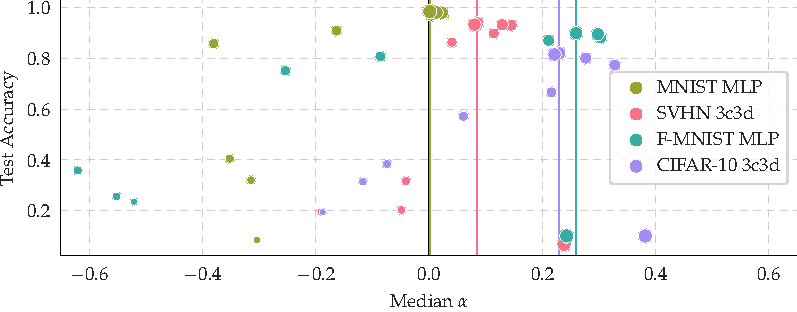
\includegraphics[width=\linewidth]{../repos/cockpit-paper/fig/07_learning_rate_selection/output/median_alpha_vs_performance_thesis-wide}
	\end{center}
  \vspace{-2ex}
	\caption{\textbf{Test accuracy as a function of standardized step size
      $\alpha$}. For four \deepobs problems (see \Cref{cockpit::app:benchmarks}), final
    test accuracy is shown versus the median $\alpha$-value over the entire
    training. Marker size indicates the magnitude of the raw learning rate,
    marker color identifies tasks (see legend). For each problem, the
    best-performing setting is highlighted by a vertical colored line.}
	\label{cockpit::fig:alpha_exp}
\end{figure*}

Across multiple optimization problems, we observe, perhaps surprisingly, that
the best runs and indeed all good runs have a median $\alpha>0$
(\Cref{cockpit::fig:alpha_exp}). This illustrates a fundamental difference between
stochastic optimization, as is typical for machine learning, and classic
deterministic optimization. Instead of locally stepping ``to the valley floor''
(optimal in the deterministic case), stochastic optimizers should
\emph{overshoot} the valley somewhat. This need to ``surf the walls'' has been
hypothesized before \citep[e.g.][]{wu2018understanding,xing2018walk} as a property of neural
network training. Frequently, learning rates are adapted during training, which
fits with our observation about positive $\alpha$-values: ``overshooting''
allows fast early progression towards areas of lower loss, but it does not yield
convergence in the end. Real-time visualizations of the training state, as
offered by \cockpit, can augment these fine-tuning processes.

\Cref{cockpit::fig:alpha_exp} also indicates a major challenge preventing simple
automated tuning solutions: the optimal $\alpha$-value is problem-dependent, and
simpler problems, such as a multi-layer perceptron (\mlp) on \mnist
\citep{lecun1998gradient}, behave much more similar to classic optimization problems.
Algorithmic research on small problems can thus produce misleading conclusions.
The figure also shows that the $\alpha$-gauge is not sufficient by itself:
extreme overshooting with a too-large learning rate leads to poor performance,
which however can be prevented by taking additional instruments into account.
This makes the case for the cockpit metaphor of increasing interpretability from
several instruments in conjunction. By combining the $\alpha$-instrument with
other gauges that capture the local geometry or network dynamics, the user can
better identify good choices of the learning rate and other hyperparameters.

%%% Local Variables:
%%% mode: latex
%%% TeX-master: "../thesis"
%%% End:


\section{Showcase}\label{cockpit::sec:showcase}
Having introduced the tool, we can now return to \Cref{cockpit::fig:showcase}
for a closer look. The figure shows a snapshot from training the \allcnnc
\citep{springenberg2015striving} on \cifarhun using \sgd with a cyclic learning
rate schedule (bottom left panel). Diagonal curvature instruments are configured
to use an MC approximation to save run time (here, $C=100$, compare
\Cref{cockpit::sec:benchmark}).

A glance at all panels shows that the learning rate schedule is reflected in the
metrics. However, the instruments also provide insights into the early phase of
training (first $\sim100$ iterations), where the learning rate is still
unaffected by the schedule: there, the loss plateaus and the optimizer takes
relatively small steps (compared to later, as can be seen in the small gradient
norms, and small distance from initialization). Based on these low-cost
instruments, one may thus at first suspect that training was poorly initialized;
but training indeed succeeds after iteration 100! Viewing \cockpit entirely
though, it becomes clear that optimization in these first steps is not stuck at
all: while loss, gradient norms, and distance in parameter space remain almost
constant, curvature changes, which expresses itself in a clear downward trend of
the maximum Hessian eigenvalue (top right panel).

The importance of early training phases has recently been hypothesized
\citep{frankle2020early}, suggesting a logarithmic timeline. Not only does our
showcase support this hypothesis, but it also provides an explanation from the
curvature-based metrics, which in this particular case are the only meaningful
feedback in the first few training steps. It also suggests monitoring training
at log-spaced intervals. \cockpit provides the flexibility to do so, indeed,
\Cref{cockpit::fig:showcase} has been created with log-scheduled tracking events.

As a final note, we recognize that the approach taken here promotes an amount of
\emph{manual} work (monitoring metrics, deliberately intervening, \etc) that may
seem ironic and at odds with the paradigm of automation that is at the heart of
machine learning. However, we argue that this might be what is needed at this
point in the evolution of the field. Deep learning has been driven notably by
scaling compute resources \citep{thompson2020computational}, and fully automated
one-shot training may still be some way out. To develop better training methods,
researchers, not just users, need \emph{algorithmic} interpretability and
explainability: direct insights and intuition about the processes taking place
``inside'' neural nets. To highlight how \cockpit might provide this, we
contrast in \Cref{cockpit::app:convex-problems} the view of two convex \deepobs
problems (noisy quadratic \& logistic regression on \mnist). In both cases, the
instruments behave differently compared to the deep learning problem in
\Cref{cockpit::fig:showcase}. In particular, the gradient norm increases (left
column, bottom panel) during training, and individual gradients become less
scattered (center column, top panel). This is diametrically opposed to the
convex problems and shows that deep learning differs even qualitatively from
well-understood optimization problems.

%%% Local Variables:
%%% mode: latex
%%% TeX-master: "../thesis"
%%% End:


\section{Benchmark}\label{cockpit::sec:benchmark}
\Cref{cockpit::sec:experiments} made a case for \cockpit as an effective debugging and
tuning tool. To make the library useful in practice, it must also have limited
computational cost. We now show that it is possible to compute all quantities at
reasonable overhead. The user can control the absolute cost along two
dimensions, by reducing the number of instruments, or by reducing their update
frequency.

All benchmark results show \sgd without momentum. \cockpit's quantities,
however, work for generic optimizers and can mostly be used identically without
increased costs. One current exception is \inlinecode{Alpha} which can be
computed more efficiently given the update rule.\sidenote{This is currently
  implemented for vanilla \sgd. Otherwise, \cockpit falls back to a less
  efficient scheme.}

\subsubsection{Complexity Analysis}

Computing more information adds computational overhead, of course. However,
recent work \citep{dangel2020backpack} has shown that first-order information,
like distributional statistics on the batch gradients, can be computed on top of
the mean gradient at little extra cost. Similar savings apply for most
quantities in \Cref{cockpit::tab:overview-quantities}, as they are
\mbox{(non-)linear} transformations of individual gradients. A subset of
\cockpit's quantities also uses second-order information from the Hessian
diagonal. For ReLU networks on a classification task with $C$ classes, the
additional work is proportional to $C$ gradient backpropagations (\ie $C=10$ for
\cifarten, $C=100$ for \cifarhun). Parallel processing can, to some extent,
process these extra backpropagations in parallel without significant overhead.
If this is no longer possible, we can fall back to a Monte Carlo (MC) sampling
approximation, which reduces the number of extra backprop passes to the number
of samples (1 by default).\sidenote{An MC-sampled approximation of the
  Hessian/generalized Gauss-Newton has been used in \Cref{cockpit::fig:showcase}
  to reduce the prohibitively large number of extra backprops on \cifarhun
  ($C=100$).}

While parallelization is possible for the gradient instruments, computing the
maximum Hessian eigenvalue is inherently sequential. Similar to
\citet{yao2020pyhessian}, we use matrix-free Hessian-vector products by
automatic differentiation \citep{pearlmutter1994fast}, where each product's
costs are proportional to one gradient computation. Regardless of the underlying
iterative eigensolver, multiple such products must be queried to compute the
spectral norm (the number depends on the spectral gap to the second-largest
eigenvalue).

\subsubsection{Run Time Benchmark}

\Cref{cockpit::fig:benchmark-instruments} shows the wall-clock computational
overhead for individual instruments (details in
\Cref{cockpit::app:benchmarks}).\sidenote{To improve readability, we exclude
  \inlinecode{HessMaxEV} here, because its overhead is large compared to other
  quantities. Surprisingly, we also observed significant cost for the 2D
  histogram on GPU. It is caused by an implementation bottleneck for histogram
  shapes observed in deep models. We thus also omit \inlinecode{GradHist2d}
  here, as we expect it to be eliminated with future implementations (see
  \Cref{cockpit::app:run-time-benchmarks} for a detailed analysis and further
  benchmarks). Both quantities, however, are part of the benchmark shown in
  \Cref{cockpit::fig:benchmark_heatmap}.} As expected, byproducts are virtually
free, and quantities that rely solely on first-order information add little
overhead (at most roughly 25\,\% on this problem). Thanks to parallelization,
the ten extra backward passes required for Hessian quantities reduce to less
than 100\,\% overhead. Individual overheads also do not simply add up when
multiple quantities are tracked, because quantities relying on the same
information share computations.

\begin{figure*}
  \centering
  \begin{subfigure}[t]{0.6\linewidth}
    \centering
    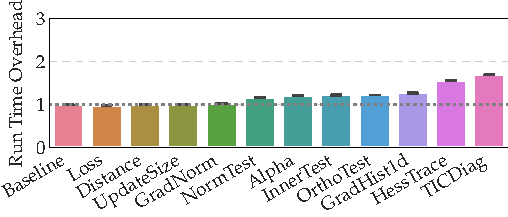
\includegraphics[width=\linewidth]{../repos/cockpit-paper/fig/01_benchmark/output/fig_individual/benchmark_cifar10_3c3d_cuda_thesis-wide}
    \caption{Overhead \cockpit instruments}
    \label{cockpit::fig:benchmark-instruments}
  \end{subfigure}
  \hfill
  \begin{subfigure}[t]{0.35\linewidth}
    \centering
    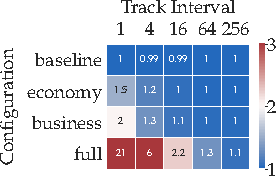
\includegraphics[width=\linewidth]{../repos/cockpit-paper/fig/01_benchmark/output/fig_grid/benchmark_cifar10_3c3d_cuda_thesis-wide}
    \caption{Overhead \cockpit configurations}
    \label{cockpit::fig:benchmark_heatmap}
  \end{subfigure}
  \caption{\textbf{Run time overhead for individual \cockpittitle instruments
      and configurations} as shown on \cifarten \threecthreed on a GPU.
    \subfigref{cockpit::fig:benchmark-instruments} The run time overheads for
    individual instruments are shown as multiples of the \emph{baseline} (no
    tracking). Most instruments add little overhead. This plot shows the
    overhead in one iteration, determined by averaging over multiple iterations
    and random seeds. \subfigref{cockpit::fig:benchmark_heatmap} Overhead for
    different \cockpit configurations. Adjusting the tracking interval and
    re-using the computation shared by multiple instruments can make the
    overhead orders of magnitude smaller. Blue fields mark settings that allow
    tracking without doubling the training time.}
  \label{cockpit::fig:benchmark}
\end{figure*}

To allow a rough cost control, \cockpit currently offers three configurations,
called \inlinecode{``economy''}, \inlinecode{``business''}, and
\inlinecode{``full''}, in increasing order of cost
(\Cref{cockpit::tab:overview-quantities}). As a basic guideline, we consider a
factor of two to be an acceptable limit for the increase in training time and
benchmark the configurations' run times for different tracking intervals.
\Cref{cockpit::fig:benchmark_heatmap} shows a run time matrix for the \cifarten
\threecthreed problem, where settings that meet this limit are set in blue (more
problems including \imagenet are shown in \Cref{cockpit::app:benchmarks}).
Speedups due to shared computations are easy to read off: summing all the
individual overheads shown in \Cref{cockpit::fig:benchmark-instruments} would
result in a total overhead larger than 200\,\%, while the joint overhead
(\textit{business}) reduces to 140\,\%. The \textit{economy} configuration can
easily be tracked at every step of this problem and stay well below our
threshold of doubling the execution time. \cockpit's full view, shown in
\Cref{cockpit::fig:showcase}, can be updated every $64$-th iteration without a
major increase in training time (this corresponds to about five updates per
epoch). Finally, tracking any configuration about once per epoch---which is
common in practice---adds overhead close to zero (rightmost column).

This good performance is largely due to the efficiency of the \backpack package
\citep{dangel2020backpack}, which we leverage with custom and optimized modification,
that compacts information layer-wise and then discards unneeded buffers. Using
layer-wise information (\Cref{cockpit::sec:vanishing_gradient_exp}) scales better to
large networks, where storing the entire model's individual gradients all at
once becomes increasingly expensive (see \Cref{cockpit::app:benchmarks}). To the best of
our knowledge, many of the quantities in \Cref{cockpit::tab:overview-quantities},
especially those relying on individual gradients, have only been explored on
rather small problems. With \cockpit they can now be accessed at a reasonable
rate for deep learning models outside the toy problem category.

%%% Local Variables:
%%% mode: latex
%%% TeX-master: "../thesis"
%%% End:


\section{Conclusion}\label{cockpit::sec:conclusion}
Contemporary machine learning, in particular deep learning, remains a craft and
an art. High dimensionality, stochasticity, and non-convexity require constant
tracking and tuning, often resulting in a painful process of trial and error.
When things fail, popular performance measures, like the training loss, do not
provide enough information by themselves. These metrics only tell \emph{whether}
the model is learning, but not \emph{why}. Alternatively, traditional debugging
tools can provide access to individual weights and data. However, in models
whose power only arises from possessing myriad weights, this approach is
hopeless, like looking for the proverbial needle in a haystack.

To mitigate this, we proposed \cockpit, a practical visual debugging tool for
deep learning. It offers instruments to monitor the network's internal dynamics
during training, in real-time. In its presentation, we focused on two crucial
factors affecting user experience: Firstly, such a debugger must provide
meaningful insights. To demonstrate \cockpit's utility, we showed how it can
identify bugs where traditional tools fail. Secondly, it must come at a feasible
computational cost. Although \cockpit uses rich second-order information,
efficient computation keeps the necessary run time overhead cheap. The
open-source \pytorch package can be added to many existing training loops.

Obviously, such a tool is never complete. Just like there is no perfect
universal debugger, the list of current instruments is naturally incomplete.
Further practical experience with the tool, for example in the form of a future
larger user study, could provide additional evidence for its utility. However,
our analysis shows that \cockpit provides useful tools and extracts valuable
information presently not accessible to the user. We believe that this improves
algorithmic interpretability -- helping practitioners understand how to make
their models work -- but may also inspire new research. The code is designed
flexibly, deliberately separating the computation and visualization. New
instruments can be added easily and also be shown by the user's preferred
visualization tool, \eg \tensorboard. Of course, instead of just showing the
data, the same information can be used by novel algorithms directly,
side-stepping the human in the loop.

%%% Local Variables:
%%% mode: latex
%%% TeX-master: "../thesis"
%%% End:


\section*{Acknowledgments}
The authors gratefully acknowledge financial support by the European Research
Council through ERC StG Action 757275 / PANAMA; the DFG Cluster of Excellence
“Machine Learning - New Perspectives for Science”, EXC 2064/1, project number
390727645; the German Federal Ministry of Education and Research (BMBF) through
the Tübingen AI Center (FKZ: 01IS18039A); and funds from the Cyber Valley
Initiative of the Ministry for Science, Research and Arts of the State of
Baden-Württemberg. Moreover, the authors thank the International Max Planck
Research School for Intelligent Systems (IMPRS-IS) for supporting Felix Dangel
and Frank Schneider. Further, we are grateful to Agustinus Kristiadi, Alexandra
Gessner, Christian Fröhlich, Filip de Roos, Jonathan Wenger, Julia Grosse, Lukas
Tatzel, Marius Hobbhahn, and Nicholas Krämer for providing feedback to the
manuscript.

%%% Local Variables:
%%% mode: latex
%%% TeX-master: "../thesis"
%%% End:
